\documentclass{report}

% -------- Packages --------

%%%%% These are the default packaes loaded by the UCL MSc Thesis
\usepackage{setspace}
%\usepackage{subfigure}

\pagestyle{plain}
\usepackage{amssymb,graphicx,color}
\usepackage{amsfonts}
\usepackage{latexsym}
\usepackage{a4wide}
\usepackage{amsmath}

%%%%%%

% This package just gives you a quick way to dump in some sample text.
% You can remove it -- it's just here for the examples.
\usepackage{blindtext}

% This package means empty pages (pages with no text) won't get stuff
%  like chapter names at the top of the page. It's mostly cosmetic.
\usepackage{emptypage}

% The graphicx package adds the \includegraphics command,
%  which is your basic command for adding a picture.
% \usepackage{graphicx}

% This command is provided by the graphicx package, and 
%  controls the default dpi resolution of images you use.
%  72 is the default, but 300 is more normal, and 600 is
%  as good as you can expect to be able to get on normal paper.
% \pdfimageresolution=300


% The float package improves LaTeX's handling of floats,
%  and also adds the option to *force* LaTeX to put the float
%  HERE, with the [H] option to the float environment.
\usepackage{float}

% The amsmath package enhances the various ways of including
%  maths, including adding the align environment for aligned
%  equations.
% \usepackage{amsmath}

% Use these two packages together -- they define symbols
%  for e.g. units that you can use in both text and math mode.
\usepackage{gensymb}
\usepackage{textcomp}
% You may also want the units package for making little
%  fractions for unit specifications.
%\usepackage{units}


% The setspace package lets you use 1.5-sized or double line spacing.
% \usepackage{setspace}
% \setstretch{1.5}

% That just does body text -- if you want to expand *everything*,
%  including footnotes and tables, use this instead:
%\renewcommand{\baselinestretch}{1.5}


% PGFPlots is either a really clunky or really good way to add graphs
%  into your document, depending on your point of view.
% There's waaaaay too much information on using this to cover here,
%  so, you might want to start here:
%   http://pgfplots.sourceforge.net/
%  or here:
%   http://pgfplots.sourceforge.net/pgfplots.pdf
%\usepackage{pgfplots}
%\pgfplotsset{compat=1.3} % <- this fixed axis labels in the version I was using

% PGFPlotsTable can help you make tables a little more easily than
%  usual in LaTeX.
% If you're going to have to paste data in a lot, I'd suggest using it.
%  You might want to start with the manual, here:
%  http://pgfplots.sourceforge.net/pgfplotstable.pdf
%\usepackage{pgfplotstable}

% These settings are also recommended for using with pgfplotstable.
%\pgfplotstableset{
%	% these columns/<colname>/.style={<options>} things define a style
%	% which applies to <colname> only.
%	empty cells with={--}, % replace empty cells with '--'
%	every head row/.style={before row=\toprule,after row=\midrule},
%	every last row/.style={after row=\bottomrule}
%}


% The mhchem package provides chemistry formula typesetting commands
%  e.g. \ce{H2O}
%\usepackage[version=3]{mhchem}

% And the chemfig package gives a weird command for adding Lewis 
%  diagrams, for e.g. organic molecules
%\usepackage{chemfig}

% The linenumbers command from the lineno package adds line numbers
%  alongside your text that can be useful for discussing edits 
%  in drafts.
% Remove or comment out the command for proper versions.
%\usepackage[modulo]{lineno}
% \linenumbers 


% Alternatively, you can use the ifdraft package to let you add
%  commands that will only be used in draft versions
%\usepackage{ifdraft}

% For example, the following adds a watermark if the draft mode is on.
%\ifdraft{
%  \usepackage{draftwatermark}
%  \SetWatermarkText{\shortstack{\textsc{Draft Mode}\\ \strut \\ \strut \\ \strut}}
%  \SetWatermarkScale{0.5}
%  \SetWatermarkAngle{90}
%}


% The multirow package adds the option to make cells span 
%  rows in tables.
\usepackage{multirow}


% Subfig allows you to create figures within figures, to, for example,
%  make a single figure with 4 individually labeled and referenceable
%  sub-figures.
% It's quite fiddly to use, so check the documentation.
%\usepackage{subfig}

% The natbib package allows book-type citations commonly used in
%  longer works, and less commonly in science articles (IME).
% e.g. (Saucer et al., 1993) rather than [1]
% More details are here: http://merkel.zoneo.net/Latex/natbib.php
% \usepackage{natbib}

% The bibentry package (along with the \nobibliography* command)
%  allows putting full reference lines inline.
%  See: 
%   http://tex.stackexchange.com/questions/2905/how-can-i-list-references-from-bibtex-file-in-line-with-commentary
\usepackage{bibentry} 

% The isorot package allows you to put things sideways 
%  (or indeed, at any angle) on a page.
% This can be useful for wide graphs or other figures.
%\usepackage{isorot}

% The caption package adds more options for caption formatting.
% This set-up makes hanging labels, makes the caption text smaller
%  than the body text, and makes the label bold.
% Highly recommended.
\usepackage[format=hang,font=small,labelfont=bf]{caption}

% If you're getting into defining your own commands, you might want
%  to check out the etoolbox package -- it defines a few commands
%  that can make it easier to make commands robust.
\usepackage{etoolbox}

% For code
\usepackage[cache=false, outputdir=_build]{minted}

% Dashed lines in some tables
\usepackage{arydshln}

% For tables with multiple columns 
\usepackage{booktabs}

% For inline lists
\usepackage[inline]{enumitem}

% Hyperlinks for references
\usepackage{hyperref}

% Set up spaces between captions
\captionsetup{belowskip=15pt,aboveskip=8pt}

% Ticks and crosses
\usepackage{pifont}% http://ctan.org/pkg/pifont
\newcommand{\cmark}{\ding{51}}%
\newcommand{\xmark}{\ding{55}}%

% Algorithms
% \usepackage{algorithm}
\usepackage[ruled]{algorithm}
\usepackage{algpseudocode}
% \usepackage{algorithmic}

% Create a new environment
\newenvironment{tight_enumerate}{
\begin{enumerate}
  \setlength{\itemsep}{0pt}
  \setlength{\parskip}{0pt}
}{\end{enumerate}}

\bibliographystyle{unsrt}

\title{     
    { 
\includegraphics[scale=.5]{ucl_logo.png} \\}
    { \Huge Project \\ }
    { \large Optional Subtitle \\}
}

\date{Submission date: Day Month Year}

\author{
    Eric Hambro
    \thanks{ 
        {\bf Disclaimer:}
        This report is submitted as part requirement for the Machine Learning MSc at UCL. 
        It is substantially the result of my own work except where explicitly indicated in the text.
        \emph{Either:} The report may be freely copied and distributed provided the source is explicitly acknowledged
        \newline  %% \\ screws it up
        \emph{Or:}\newline
        The report will be distributed to the internal and external examiners, but thereafter may not be copied or distrbuted except with permission from the author.
    }
    \\ \\
    MSc Machine Learning\\ \\
    Prof Sebastian Riedel
}

\nobibliography*

\begin{document}
 
\maketitle
\makedeclaration

\begin{abstract} % 300 word limit
My research is about stuff.

It begins with a study of some stuff, and then some other stuff and things.

There is a 300-word limit on your abstract.
\end{abstract}

\begin{acknowledgements}
Acknowledge all the things!
\end{acknowledgements}

\setcounter{tocdepth}{2} 
% Setting this higher means you get contents entries for
%  more minor section headers.

\tableofcontents
\listoffigures
\listoftables


\chapter{Introductory Material}
\label{chapterlabel1}

\section{Motivation} % (fold)
\label{sec:motivation}


Code documentation is a tedious and important part of writing and reading industrial code. It can be varied and describe circuituous or irrelevant information about the function. In this paper we present a new dataset of argument functions and their source code and descriptions, and show that the best methods of training data involved the use of source code as well as named variables. 
% section motivation (end)

\section{Problem Formulation} % (fold)
\label{sec:problem_formulation}

\begin{itemize}
    \item in ideal world translate from code to english (semantic parsing)
    \item this neglects the idiomatic naturalness of big code (big code and naturalness)
    \item we seek a model of translation of elements of code and other information into natural language
    \item our investigation finds a new dataset where the link between semantic meaning, naturalness and natural language is very strong. 
    \item we investigated this dataset using machine translation techniques and found blah
\end{itemize}
% section problem_formulation (end)
 
\section{Related Work} % (fold)

This could be a very big section. 

\subsubsection{Naturalness to English} % (fold)
\label{ssub:naturalness_to_english}

Here we talk a bit about the big code and naturalness papers. Allamanis etc al.

Papers such as: extreme summarization of source code, graph neural network, etc..

We reference other datasets that are available, and analyse the problems with them


\subsubsection{Code to English} % (fold)
\label{ssub:code_to_english}

Here we talk a bit about structured language to english. Semantic parsing. We talk about the datasets and the very limited fields. (Pointer networks)
% subsubsection naturalness_to_english (end)

We talk about maybe some english to code methods:
* SQL
* program synthesis

\subsection{Other Investigations with Code} % (fold)
\label{sub:other_investigations_with_code}

Here we refer to code to vec.
And maybe some more stuff
% subsection other_investigations_with_code (end)

\label{sec:related_work}

% section related_work (end)

 % subsection subsection_name (end) 

% Some stuff about things. \cite{example-citation} Some more things. 

% Inline citation: \bibentry{example-citation}

% This is just a bare misdnimum to get started.  There is unlimited guidance on using latex, e.g. {\tt https://en.wikibooks.org/wiki/LaTeX}.   You are still responsible to check the detailed requirements of a project, including formatting instructions, see \\
% {\tt https://moodle.ucl.ac.uk/pluginfile.php/3591429/mod\_resource/content/7/UGProjects2017.pdf}.
% Leave at least a line of white space when you want to start a new paragraph.

% Mathematical expressions are placed inline between dollar signs, e.g. $\sqrt 2, \sum_{i=0}^nf(i)$, or in display mode
% \[ e^{i\pi}=-1\] and another way, this time with labels,
% \begin{align}
% \label{line1} A=B\wedge B=C&\rightarrow A=C\\
% &\rightarrow C=A\\
% \intertext{note that}
% n!&=\prod_{1\leq i\leq n}i \\
% \int_{x=1}^y \frac 1 x \mathrm{d}x&=\log y
% \end{align}
% We can refer to labels like this \eqref{line1}. 


\chapter{Literature Survey}
\label{literature_survey}

\begin{itemize}
    \item Code has become an integral part of the underpinnings of modern life. This seems likely to continue if not accelerate.
    \item However the number of people who can read \& write code remains small as a percentage of the population. 
    \item Tools that can help either read, write or analyse code hold the potential to provide great value, for both professional software engineers, and also non-coders.
    \item With the proliferation of industry quality open source code, a great deal of research has gone into the field of trying do this translation.
\end{itemize}

\section{Big Code \& Naturalness} % (fold)

\subsection{The Naturalness Hypothesis} % (fold)
\label{ssub:the_naturalness_hypothesis}

% subsubsection the_naturalness_hypothesis (end)
\begin{itemize}
    \item How does code vary from natural language?
        \begin{itemize}
            \item formal, executable, brittle, unique sentences, neologisms, reuse, ambiguity, two channels vs one channel
        \end{itemize}
    \item What similarities are there?
        \begin{itemize}
            \item naming, objects are anchored (metaphors of OOP), idiomatic writing, patterns
        \end{itemize}
    \item How does this lead to the naturalness hypothesis
        \begin{itemize}
            \item latter patterns are ignored by the computer yet present in large datasets \textbf{CITE}. 
            therefore seem to indicate that asignificant part of code is communication for other humans, not the computer - cf literate programming Knuth
            \item \textbf{Naturalness Hypothesis} - ``Software is a form of human communications; software corpora have a similar statistical properties to natural language coprora; and theses properties can be exploited to build better software tools'' 
            \item The implication is therefore we can make use of the body of work and probabilistic models on natural language and transfer to code.
        \end{itemize}
\end{itemize}


\subsection{Related Work} % (fold)
\label{ssub:related work}

A number of different people have attempted to use probabilistic models for language, in this fields ranging in a variety of tasks:

Big Code papers:
* predicting program properties from big code
* mining semantic idiom loops from big code
* sumarazing source code with attention ,
* convlutional attention network
* graph to spot bugs

Also significant work inolving natural laguage & code
* semantic language model
* phrase based statistical translation
* predicting program code

Differnet approachs:
* program embeddings to studet code
* grap ealier
* code2vec

Traditional Machine Translation approaches
* Bahdnause
* Seq to seq

Existing datasets
* allamanis


A number of other papers are working on 


related topics: source code summarization x 2, 

\textbf{Generating English}
\begin{itemize}
    \item 
    \item Extreme summarization of source code (allamanis)
    \item Summarization using neural attention model
    \item Preidcting Programming COmmets
\end{itemize}

\textbf{Observing Patterns in Code}
\begin{itemize}
    \item Allamanis graph paper
    \item Extracting patterns/idioms from source code (allamanis)
    \item Program properties from big code
\end{itemize}

\textbf{Representation of Code}
\begin{itemize}
    \item Code2Vec
    \item Code embeddings the other paper
\end{itemize}

\textbf{Datasets}
\begin{itemize}
    \item Edinburgh NLP
    \item IFTTT
    \item Django 
\end{itemize}


% \subsection{Useful datasets} % (fold)
% \label{ssub:existing_datasets}

% Here we talk a bit about structured language to english. Semantic parsing. We talk about the datasets and the very limited fields. (Pointer networks)
% % subsubsection naturalness_to_english (end)

% We talk about maybe some english to code methods:
% * SQL
% * program synthesis

% \subsection{Other Investigations with Code} % (fold)
% \label{sub:other_investigations_with_code}

% Here we refer to code to vec.
% And maybe some more stuff
% % subsection other_investigations_with_code (end)

% \label{sec:related_work}
\chapter{Theoretical Background}
\label{theoreticalbackground}




\section{Neural Network Translation Models} % (fold)
\label{sec:lstm}

\subsection{Recurrent Neural Networks for Language Modelling} % (fold)
\label{sub:recurrent_neural_networks}

\subsection{Sequence to Sequence Architectures} % (fold)
\label{sub:sequence_to_sequence_architectures}

\subsection{Attention} % (fold)
\label{sub:attention}

\subsection{Backpropagation} % (fold)
\label{sub:backpropagation}
% subsection sequence_to_sequence_architectures (end)
% subsection recurrent_neural_networks (end)

\blindtext

\section{Structure of Code} % (fold)
\label{sec:translating_code}

\subsection{Function Declarations} % (fold)
\label{sub:function_declarations}

\subsection{Abstract Syntax Trees} % (fold)
\label{sub:abstract_syntax_trees}


% subsection working_with_rnns_&_tress (end)
% subsubsection encoding_trees (end)
% subsection abstract_syntax_trees (end)

\blindtext

\chapter{TheDataset}
\label{the_dataset}

\section{Method of Collection} % (fold)
\label{sec:method_of_collection}

% section method_of_collection (end)

\section{Structure of Dataset} % (fold)
\label{sec:structure_of_dataset}

% section structure_of_dataset (end)

\section{Analysis of Data} % (fold)
\label{sec:analysis_of_data}

\subsection{Statistical Analysis of Natural Language} % (fold)
\label{sub:statistical_analysis_of_natural_language}

% subsection statistical_analysis_of_natura_language (end)

\subsection{Statistical Analysis of Code} % (fold)
\label{sub:statistical_analysis_of_code}

% subsection statistical_analysis_of_code (end)

\subsection{Qualitative Analysis of Dataset} % (fold)
\label{sub:qualitative_analysis_}

% subsection qualitative_analysis_ (end)
% section analysis_of_data (end)
\chapter{Method}
\label{the_models}

% We focused on the signature because of the important nature of this section of the code. 
% In langugages such as C++, the signature of function may be all that is presented to the user of a third-party library, when using that library. 
% Therefore being able to generate reasonable descriptions from signature items alone would already be of value. 
% This does not seem an unrealistic target, since good developer practice often involves giving insightful names to variables and functions\footnote{https://github.com/google/styleguide/blob/gh-pages/pyguide.md\#s3.16-naming}.


\section{Overview}

In our investigations we focus on two main aspects of the code to generate descriptions for our arguments. 
These are the names in the function's signature, and the \textit{variable path-contexts} (VPCs) in the function's AST. 


In our experiments, we model the names of the signature as sequences of characters. We do this to capture the fact that variable and function names can often be composite and abbreviated - e.g. \mintinline[]{python}{web_ctx}. 
In this case both parts of the name might indicate a different clue to the argument:  the  \mintinline[]{python}{web} prefix may indicate a use in the internet domain; the \mintinline[]{python}{ctx} suffix may indicate a context object. 
In designing our models, we aim to pick up these patterns and conventions on the character-level.

We also focused on generating descriptions solely from the argument's VPCs. We feel that this most robust way of drawing inferences from the code, as it only examines instructions given directly to the computer. 
Any inferences here would be invariant under transformations such as renaming of variable. 
We hoped that by examining all the VPCs present for an argument, the model would learn representation for variables that indicate common usage (such as which methods are called on it), or perhaps even type.

% We chose to model this information as bag of modified `path-contexts' \cite{alon_general_2018} relevant to each variable. This would allow us to extract only the relevant sections of code pertintent to our chosen argument from the AST. 
% We hoped our models would then be able to learn which modified `path-contexts' are most informative, picking out the most relevant sections of code.

We prepared four models to investigate these data: A Rote Learner to act as baseline for our investigations; a character-level Seq2Seq Model to investigate the signature names; an original Code2Vec Decoder model to investigate the VPCs; and a Code2Vec + Seq2Seq Model to investigate both inputs combined.

The rest of this section is dedicated to presenting each of these models, summarised in Table \ref{tab:our_models_capability}, along with the  tokenization methods to obtain our data.



\begin{table}[tb]
    \centering

    \begin{tabular}{c  c  c}
          Model & Uses Signature Data & Uses VPC Data \\ 
    \hline
    Rote Learner & \checkmark & \checkmark \\
    Seq2Seq Decoder & \checkmark & \\
    Code2Vec Decoder &    &  \checkmark \\
    Code2Vec + Seq2Seq Decoder& \checkmark & \checkmark \\
    \hline
    \end{tabular}
    \caption{Overview of Our Models}
    \label{tab:our_models_capability}
\end{table}











\section{The Models}

\subsection{Rote Learner Model} % (fold)
\label{sec:rote_learner_model}

Our Rote Learner model was designed to act as a strong benchmark in all our investigations. 
It was designed according to a simple principle: \textit{the Rote Learner generates a description from a test point by returning in full a random description from a list of best-matching training point.}
It is defined formally in Algorithm \ref{alg:rote_learner_general}. 

The benefit of this model is that the definition of `best-matching' can then be changed according to the modality of the input data. In the sections below we present a brief description of these matching algorithms, with an appendix displaying each algorithm in pseudocode. A summary of these matching algorithms is presented in Table \ref{tab:matching_summary}, 

\begin{algorithm}
    \caption{The general Rote Learner algorithm }
    \label{alg:rote_learner_general}
    \begin{algorithmic}
        \Procedure{GenerateDescription}{$t$}\Comment{Generate a description for test argument $t$ }
        \State $\mathcal{M} \gets \text{BestMatchingSet}(t, training\_points)$
        \State $x \gets \text{RandomChooseOne}(\mathcal{M})$
        \State $d \gets \text{GetDescription}(x)$
        \State \textbf{return} $d$
        \EndProcedure
    \end{algorithmic}
\end{algorithm}

\begin{enumerate}
    \item \textbf{NCharacter-Gram Overlap} \textit{(Sig. Data)} \\This matching criterion was used for function signature data, and so operates on sequences of characters. It compiles a list of the training points which have the longest n character overlap with the test data point (or the longest common substring). If the same point has two of such overlaps, it is included twice, and so forth. This pseudo code is presented in Algorithm \ref{alg:ngram_overlap}.
    \item \textbf{Proportional Contexts} \textit{(VPC Data)}\\This criterion matches VPCs by treating each VPC as an atomic unit. For each VPC within the test point, the criterion finds all the training points with the same VPC. It combines these into one list, returns this list. Naturally, the list may have duplicates of the same training point. This is equivalent to choosing the training points proportionally to how often they have an overlapping VPC with the test point. The pseudocode is presented in Algorithm \ref{alg:context_algorithm} 
    \item \textbf{Max Contexts} \textit{(VPC Data)}\\This criterion takes the list output by the \textbf{Proportional Context} criterion, and only chooses the training points that appear most frequently in the list. This is equivalent to choosing the training points that have the greatest number of overlapping path-contexts with the test point. The pseudocode is also presented in Algorithm \ref{alg:context_algorithm} 
    \item \textbf{Proportional SubContexts} \textit{(VPC Data)}\\This criterion also match VPCs of the data, but treats each VPC as sequence of nodes. Specifically, as it creates $q = p{downarrow}x_f$ and treats the new path, $q$, as the sequence of nodes and arrows that compose it. This allows it to match subpaths. The matching criterion takes the test point, and for each VPC within it, finds the training VPC with the longest subsequences that matches it. It collects the corresponding datapoints to these paths and combines them into one list. It then returns this list. This is equivalent to choosing the training points that best match each VPC in the test point, proportionally to how often they are the best match. The pseudocode is presented in Algorithm \ref{alg:sub_context_algorithm} 
    \item\textbf{Max SubContexts} \textit{(VPC Data)}\\The matching criterion takes the list output by the \textbf{Proportional SubContext}, and only chooses the training points that appear most frequently in the list. This is equivalent to choosing the training points that most often are the best match for all path-contexts of the test. The pseudocode is presented in Algorithm \ref{alg:sub_context_algorithm} 
    \item\textbf{[Combinations]}\textit{(Sig. Data + VPC Data)} \\ Naturally these criteria can be combined across modalities to act upon combinations of the function signature and AST. In cases where this is done, the new list is simply the combination of the lists from the combined individual criteria. 
\end{enumerate}









\begin{table}[h!]
\makebox[\linewidth][c]{
    \centering

    \begin{tabular}{l c c p{9cm}}
    \hline
    BestMatchingSet & Use Sig. & Use AST & Description: \textit{choose list of training points...} \\
    \hline
    \hline
    NCharacter-Gram Overlap     & \checkmark & & 
         which have the longest n-character gram overlap with test \\
    % \hline
    % \hline
  
    Proportional Context  & & \checkmark & 
        which match each VPC in test, and combine\\
    Max Context  & & \checkmark &
        which match each VPC in test, combine, and take most frequent\\

    Proportional SubContext  & & \checkmark &
        which \textit{best-effort} match each VPC in test, and combine\\
    Max SubContext  & & \checkmark & 
        which \textit{best-effort} each VPC in test, combine, and take most frequent\\
    Combinations  &\checkmark  & \checkmark & 
        combine the lists from any two BestMatchingSets\\
    \hline

    \hline
    \end{tabular}
}

    \caption{An Summary of the BestMatchingSet algorithms we use in the experiments. For sake of simplicity, a \textit{best-effort} match here refers to the match with longest matching subsequence, when treating a VPC as one long sequence}
    \label{tab:matching_summary}
\end{table}





% These chose a description from a set of training samples by:
%     \begin{itemize}
%         \item combining samples with largest subpath overlap for each path in test, and chosing from that list. (Sub Path Proportional)
%         \item combining samples with largest subpath overlap for each path in test, and chosing from the most frequent training point(s) in that list. (Sub Path Max)
%         \item combining samples full overlap for each path in test, and chosing from that list (Full Path Proportional)
%         \item combining samples full overlap for each path in test, and chosing from the most frequent training point(s) in that list. (Full Path Max)
%     \end{itemize}








% subsection rote_learner_model (end)

\subsection{Character Level Sequence to Sequence Model} % (fold)
\label{sec:character_level_sequence_to_sequence}

The character level sequence model follows the standard formulation as found in \cite{bahdanau_neural_2014}

* What is the motivation of the seq to seq model.
* Since so much effort goes into naming of variables, shouldnt there be recognisable clues? Especially since,in many languages, function signature is all thats presented in documentation.
* \_ctx => context? conv2d in the function implies somethings?
* We therefore employ a sequence to sequence model to investigate the informativeness of function signatures



% subsection character_level_sequence_to_sequence (end)

\subsection{Code2Vec Decoder Model} % (fold)
\label{sec:code2vec_decoder_model}

* We then want to investigate purely without lexical names (overlap etc)
* We decide to present a modification on Code2Vec, that is argument specific.
* The motivtion is that this hsould be able to point out only some local parts of the model, the bits of the code that are near or important might get upweighted.


% subsection code2vec_to_sequence_model (end)

\subsection{Code2Vec + LSTM Encoder} % (fold)
\label{sub:code2vec_sequence_to_sequence}

Aim to combine these models together.Natural through 

% subsubsection code2vec_sequence_to_sequence (end)
% section combined_encoder_models (end)










\section{Tokenizations} % (fold)
\label{sec:tokenizations}

\subsection{Function Signature Data}

Tokenizations of the function signature data

\subsection{Abstract Syntax Trees Data }


\subsection{Argument Description}





% subsection evaluation_procedure (end)

% subsection tokenizing_code_features (end)

% subsubsection tokenizing_argument_descriptions (end)

% subsection tokenizing_textual_input (end)

% \subsubsection{Preparing the Data} % (fold)
% \label{ssub:Preparing the Data}

% \begin{enumerate}
%     \item All our data would come from one of the partitions of the dataset described in section \ref{sec:final_preparations}.

%     \item To tokenize variable names, function names and other arguments:
%     \begin{enumerate}
%         \item we generated a vocabulary of all possible tokens in valid python
%         \item We added separator tokens to the vocabulary, \mintinline{python}{"<SEPARATOR_1>"}
%         \item We then tokenizer as sequences of characters and adding an \mintinline{python}{"<END_OF_ARG>"} token to the end.
%     \end{enumerate}
    
%     \item To tokenize the argument descriptions:
%     \begin{enumerate}
%         \item We then generated a vocabulary for our training data by:
%         \begin{enumerate}
%             \item first generating a provisional vocabulary of tokens used more than 4 times in the training data.
%             \item if these words existed in our Glove embedding vocabulary they were added to our the final vocabulary. We used the  \mintinline{python}{glove.6B.200d.txt} file of 200d embeddings trained on 6 billion tokens for our Glove embeddings, (CITE). 
%             \item when this provisional list was exhausted we took the remaining most popular words, as defined by the Glove embedding file, to fill our final vocabulary to our designated "vocab-size"
%         \end{enumerate}
%         \item We then tokenized the descriptions by moving to lower case, removing new lines, and  tokenizing them using the nltk punkt tokenizer (\mintinline{python}{nltk.word_tokenize})
%         \item We then replaced out of vocabulary tokens with an \mintinline{python}{"<UNK>"} token, and finally bookending our descriptions with \mintinline{python}{"<START>"} and \mintinline{python}{"<END>"} tokens.
%         \item Path - seq?

%     \end{enumerate}



%     \item In cases of tokenized code: 
%      \begin{enumerate}
%          \item  In the case of tokenizing code paths, we first extracted the syntax tree from the source code, and traversed it exploring all paths between two nodes.
%          \item CONTINUE
%      \end{enumerate}

% \end{enumerate}

% Once these tokenizations were complete we were ready to train our models.

% \subsubsection{Training} % (fold)
% \label{ssub:training}


%     Our models were trained in the standard way:
%     \begin{enumerate}
%         \item The Rote Learner was trained determininstically, in this case using `ngram overlap' feature, as mentioned in\ref{sec:rote_learner_model}. It was evaluated with different random seeds 50 times on the hold out dataset.
%         \item The Seq-to-Seq model was trained using the backpropagation algorithm and adaptive momentum optimisation. The hyperparameters are presented in table X. 80 Epochs were evaluated, and the best and average scores were taken \textbf{EDIT}
%     \end{enumerate}




% \subsubsection{Evaluation} % (fold)
% \label{ssub:evaluation}

% % subsection training (end
% \begin{enumerate}



%     \item Finally when it came to evaluating our models on held-out datasets, we would ran translations on the dataset and calculated the BLEU score using the BLEU method found in \textbf{HERE}.
%     In particular BLEU scores were calculated over the whole corpus and \textbf{WHAT SMOOTHING HYPERPARAMTERS}.
%     \item It should be stressed that if a hyperparameter had to be tuned, it was always done on the validation set, with the test set untouched, until final evaluation. In the case of all neural models, the results presented are using the best hyperparameters under the validation set.

% \end{enumerate}









\chapter{Experiments and Results}
\label{experiments_and_results}


All experiments followed a similar general pattern of execution. 
This pattern of execution is described in detail in Section \ref{sec:experimental_setup}, which covers the general pipeline of the preparation, training and evaluation for each experiment.
Section \ref{sec:investigating_human_readable_channel} then describes the specific experiments and results of our investigations in to the human readable channel of code, whereas Section \ref{sec:investigating_the_computer_channel} covers the computer readable channel investivations.
The the results of the experiments combining these channels is presented in \ref{sec:investigating_combined_channels}, and further experiments into the dataset are presented in section \textbf{SECTION}


\section{Experimental Setup} % (fold)
\label{sec:experimental_setup}

\subsection{General Procedure} % (fold)
\label{sub:general_procedure}

% subsection general_procedure (end)

All our experiments were conducted in the same fashion, starting with a choice of dataset partition from Table \ref{table:thefinaldataset} that would be suitable to the investigation.
We would then tokenize the names and descriptions and other textual features, and if necessary extract the features we would from the code. 
These tokenization procedures and code extraction procedures are described in subsections \ref{sub:tokenizing_textual_input}, \ref{sub:tokenizing_argument_descriptions} and \ref{sub:tokenizing_code_features}.
After tokenization, the neural models would be trained on TESLA \textbf{GPUs}, for HOW long. 
These would evaluate performance on a dev set every epoch, and print translations.
How long did an epoch take.
When did we stop training.
Models were all evaluated by the same procedure as detailsed in section blah. 
%evaluated by assessing the BLEU, loss \& perplexity.


\subsection{Tokenizing Argument and Function Names} % (fold)
\label{sub:tokenizing_textual_input}

\subsection{Tokenizing Argument Descriptions} % (fold)
\label{sub:tokenizing_argument_descriptions}

\subsection{Tokenizing Code Features} % (fold)
\label{sub:tokenizing_code_features}

\subsection{Evaluation Procedure} % (fold)
\label{sub:evaluation_procedure}

% subsection evaluation_procedure (end)

% subsection tokenizing_code_features (end)

% subsubsection tokenizing_argument_descriptions (end)

% subsection tokenizing_textual_input (end)

% \subsubsection{Preparing the Data} % (fold)
% \label{ssub:Preparing the Data}

% \begin{enumerate}
%     \item All our data would come from one of the partitions of the dataset described in section \ref{sec:final_preparations}.

%     \item To tokenize variable names, function names and other arguments:
%     \begin{enumerate}
%         \item we generated a vocabulary of all possible tokens in valid python
%         \item We added separator tokens to the vocabulary, \mintinline{python}{"<SEPARATOR_1>"}
%         \item We then tokenizer as sequences of characters and adding an \mintinline{python}{"<END_OF_ARG>"} token to the end.
%     \end{enumerate}
    
%     \item To tokenize the argument descriptions:
%     \begin{enumerate}
%         \item We then generated a vocabulary for our training data by:
%         \begin{enumerate}
%             \item first generating a provisional vocabulary of tokens used more than 4 times in the training data.
%             \item if these words existed in our Glove embedding vocabulary they were added to our the final vocabulary. We used the  \mintinline{python}{glove.6B.200d.txt} file of 200d embeddings trained on 6 billion tokens for our Glove embeddings, (CITE). 
%             \item when this provisional list was exhausted we took the remaining most popular words, as defined by the Glove embedding file, to fill our final vocabulary to our designated "vocab-size"
%         \end{enumerate}
%         \item We then tokenized the descriptions by moving to lower case, removing new lines, and  tokenizing them using the nltk punkt tokenizer (\mintinline{python}{nltk.word_tokenize})
%         \item We then replaced out of vocabulary tokens with an \mintinline{python}{"<UNK>"} token, and finally bookending our descriptions with \mintinline{python}{"<START>"} and \mintinline{python}{"<END>"} tokens.
%         \item Path - seq?

%     \end{enumerate}



%     \item In cases of tokenized code: 
%      \begin{enumerate}
%          \item  In the case of tokenizing code paths, we first extracted the syntax tree from the source code, and traversed it exploring all paths between two nodes.
%          \item CONTINUE
%      \end{enumerate}

% \end{enumerate}

% Once these tokenizations were complete we were ready to train our models.

% \subsubsection{Training} % (fold)
% \label{ssub:training}


%     Our models were trained in the standard way:
%     \begin{enumerate}
%         \item The Rote Learner was trained determininstically, in this case using `ngram overlap' feature, as mentioned in\ref{sec:rote_learner_model}. It was evaluated with different random seeds 50 times on the hold out dataset.
%         \item The Seq-to-Seq model was trained using the backpropagation algorithm and adaptive momentum optimisation. The hyperparameters are presented in table X. 80 Epochs were evaluated, and the best and average scores were taken \textbf{EDIT}
%     \end{enumerate}




% \subsubsection{Evaluation} % (fold)
% \label{ssub:evaluation}

% % subsection training (end
% \begin{enumerate}



%     \item Finally when it came to evaluating our models on held-out datasets, we would ran translations on the dataset and calculated the BLEU score using the BLEU method found in \textbf{HERE}.
%     In particular BLEU scores were calculated over the whole corpus and \textbf{WHAT SMOOTHING HYPERPARAMTERS}.
%     \item It should be stressed that if a hyperparameter had to be tuned, it was always done on the validation set, with the test set untouched, until final evaluation. In the case of all neural models, the results presented are using the best hyperparameters under the validation set.

% \end{enumerate}

% section experimental_setup (end)

\section{Investigating Human Readable Channel} % (fold)
\label{sec:investigating_human_readable_channel}

% INVESTIGATION PURELY BASED ON NAME
\subsection{Comparing Baseline Models} % (fold)
\label{sub:comparing_baseline_models}

\subsubsection{Experiment Objective} % (fold)

As a baseline, we first wanted to investigate the informative power of simply the names of variables, with regards to different architectures of our baseline model.
We expected a reasonable signal to come from just the variable name which should be learnable by both our seq-to-seq model and rote learner. 

\subsubsection{Method \& Results} % (fold)

Since this experiment would only use the variable name to predict the descrption, we used the Reduced Random-Split Dataset listed in section.
This prevented inflation of BLEU scores due to exact matches being both in the train and validation set.

We then ran the standard tokenizations of input name on the Rote Learner, which only used the N-character-gram overlap criterion.
This was repeated 50 times, to provide an robust estimate of the standard deviation and mean BLEU scores, due to the inherent stocasticity to the model.

Then we ran a series of experiments on the basic Char-to-Seq architectures, starting from a basic seq-to-seq, then adding attention, a bidirectional encoder and finally dropout.
These best models were taken on the best BLEU scores up to 150 epochs, of training, and evaluated on the test and development set. % WHY 150

We report the BLEU scores in Table \ref{table:name_baseline} showing a strong performance from the Rote Learner of corpus level BLEU $9.03 \pm 0.32$ on validation and $10.60 \pm  0.30$. 
The Seq-to-Seq architectures initially underperformed the Rote Learner, scoring $7.76 $ and $  7.63$ on the validation and test set. However a marked improvement was seen by adding attention, as was adding the bidirectional encoder and dropout. 
The final model, with all addition beat the Rote Learner reasonably with a BLEU score of $12.46 $ and $12.72$ on validation and test set respectively.

The hyperparameters for these models are found in the Appendix, Table \ref{table:hyperparams_name_baseline}.
% ALL STOPPED at 150 EPOCHS. No improvement on best for 20 epochs, except original 146


\begin{table}[!ht]
\begin{center}
\begin{tabular}{ c | c | c }
    Model                             & BLEU (Validation)  & BLEU (Test)    \\
    \hline
    Rote Learner (x50)                & $ 9.03 \pm  0.32 $ & $ 10.60 \pm 0.27 $   \\
    \hline
    Seq to Seq                        & $ 8.97 $ & $ 8.18 $ \\
    + \textit{attention}              & $ 10.05 $ & $ 9.89 $  \\
    + \textit{bidirectional encoder}  & $ 11.76 $ & $ 12.34 $  \\
    + \textit{dropout}                & $ 12.68 $ & $ 12.72 $  \\
    \hline

    % Model                             & BLEU (Validation)  & BLEU (Test)    \\
    % \hline
    % Rote Learner (x50)                & $ 9.03242 \pm  0.31980 $ & $ 10.59658 \pm 0.26939 $   \\
    % \hline
    % Seq to Seq                        & $ 8.98624 $ & $ 8.17635 $ \\
    % + \textit{attention}              & $ 10.05134 $ & $ 9.88608 $  \\
    % + \textit{bidirectional encoder}  & $ 11.75615 $ & $ 12.34480 $  \\
    % + \textit{dropout}                & $ 12.67504 $ & $ 12.72236 $  \\
    % \hline
    % Seq to Seq                        & $ 4.60169 $ & $ 4.97880 $  \\
    % + \textit{attention}              & $ 4.81255 $ & $ 5.42022 $  \\
    % + \textit{bidirectional encoder}  & $ 3.00068 $ & $ 3.05952 $  \\
    % + \textit{dropout}                & $ 6.37864 $ & $ 6.33307 $  \\
    % \hline
\end{tabular}
\caption {Results of Experiment \ref{sub:comparing_baseline_models}: Comparing Baseline Models }
\label{table:name_baseline}
\end{center}
\end{table}



\subsubsection{Analysis} % (fold)

Most surprising of this result is the strength of the Rote Learner, despite there being no `exact matches' in the training and development sets. 
This is largely the result of there are arguments in the corpus with very similar descriptions, which may vary by only a few words. 

To investigate this we examined the predictions from the Rote Learner on the validation set. 
We evaluated the sentence level BLEU score on these, and found that although the vast majority evaluate to zero, a number of examples have a coincidental overlap in descriptions, resulting in a non negligible BLEU score. 
A random sample of these non-zero scored translations are presented in Figure \ref{tab:rotelearner_nameonly}.

With regard to the Seq-to-Seq, it is not surprising these standard additions to the seq-to-seq architecture improve the model. 
The addition of a bidirectional model adds capacity to the model by increasing the size of the hidden vector, and attention allows the model to condition sentence generation on the input, further adding complexity to the model.
The dropout also adds a regularizing effect.

It is perhaps surprising that the vanilla Seq-to-Seq struggles to outperform the Rote Learner. 
It is possible that the lack of contextualising information from attention results in an inability to learn from long description sequences that the Rote Learner can regurgitate immediately. 

However, once the attention and capacity are increased the results are explanatory.
The model synthesises similar (or even the same!) sequences of characters with their different descriptions, into a single description, which may fit better than randomly guessing from a bag of seen sequences. 

For instance, the most frequent argument, \mintinline[]{yaml}{name}, occurs in the train set 318 times with different descriptions. 
It also occurs 52 times in the validation set, again, with different descriptions. 
For each of these point the Rote Learner predicts a different description from the train set, on average scoring $0.00646 \pm 0.006$, whereas the Seq-to-Seq makes the same prediction each time, and scores $0.4029$, almost two orders of magnitude better, with the sensible average: ``name of the variable to return." 

In these cases the Seq-to-Seq model is interpolating in an overdetermined problem, and this highlights one of the advantages of neural networks in machine translation problems. 




\begin{table}
\begin{center}
\makebox[\linewidth][c]{
\begin{tabular}{l}
\hline\\

\textbf{A Random Sample of Bleu Scores $>0$ from Rote Learner on Random Split }\\\\ 


\textbf{Bleu Score}: 0.364
\textbf{Confidence}: 100.0\%  \\
\textbf{Argument}: \mintinline[]{python}{e d g e _ m a t c h}\\
\textbf{Description}: a function that returns true if the edge attribute dictionary for \\
the pair of nodes ( u1 , v1 ) in g1 and ( u2 , v2 ) in g2 should be considered equal during\\
the isomorphism test . if edge\_match is not specified then edge attributes are not considered .\\
\textbf{Prediction}: a function that returns true if the edge attribute dictionaries for\\
the pair of nodes ( $<$UNK$>$ , $<$UNK$>$ ) in $<$UNK$>$ and ( u2 , $<$UNK$>$ ) in $<$UNK$>$\\
should be considered equal during matching .\\

\\
\textbf{B}: 0.075
\textbf{C}: 11.1\%  \\
\textbf{A}: \mintinline[]{python}{u s e _ l o c k i n g}\\
\textbf{D}: ` bool ` . if true use locks for update operation .\\
\textbf{P}: an optional ` bool ` . defaults to ` true ` . an optional bool . defaults to\\
true . if true , the assignment will be protected by a lock ; otherwise the behavior is\\
undefined , but may exhibit less contention .\\
\\
\textbf{B}: 0.558
\textbf{C}: 12.5\%  \\
\textbf{A}: \mintinline[]{python}{y _ t r u e}\\
\textbf{D}: ground truth ( correct ) target values .\\
\textbf{P}: ground truth ( correct ) labels .\\
\\
\hline
\\
\end{tabular}
}
\end{center}
\caption{This is a random sample of sentence level BLEU scores that are non-zero fon the validation set for a Rote Learner}
\label{tab:rotelearner_nameonly}
\end{table}


% INVESTIGATION DIFFERENT TOKENIZATIONS
\subsection{Investigating Different Tokenizations} % (fold)
\label{sub:investigating_different_tokenizations}

\subsubsection{Experiment Objective} % (fold)

Having established a naive baseline and the validity of our neural approaches, we decided to investigate how other human names could help our translation problem.
We hypothesised that the names in the function signature could play an important role in contextualising an overdetermined or underdetermined variable name, further improving the performance of the LSTM relative to the Rote Learner.

\subsubsection{Method \& Results} % (fold)

We investigated how four different arrangements of input data would affect translation behaviour. 
These were:
just the argument name; the argument name with the function name; the argument name with co-argument names; and the argument name with both function name and co-argument names.

Once again we used the Reduced Random-Split Dataset, to prevent advantages due to duplicates, and ran the standard tokenization procedures outline in Sections X. 

As in section \ref{sub:comparing_baseline_models}, we ran 50 repetitions of the Rote Learner on these new tokenizations, to overcome the stochasiticity in their evaluations, once again using N-character-gram overlap as the matching criterion.

Then we ran four models of the Seq-to-Seq architectures, with attention, dropout and bidirectional encoders - just as the final model of section \ref{sub:comparing_baseline_models}. These ran for a maximum of 150 epochs, and the model with best BLEU score was selected. 

We report the results in Table \ref{table:tokenization}. 
In particular we note that in all cases the Rote Learner's performance improved with added information, in the best case, over three points to $12.22 \pm 0.23$ on validation and $14.34 \pm 0.21$ on test, thanks to the addition of the function name. 

The Seq-to-Seq model on the other hand benefitted less than the Rote Learner, if at all. In both tokenizations using other arguments, the model improved by approximately one point. However the tokenization involving the addition of just function name, saw a performance reduction of about 1.5 points, across both validation and test.

Although this agreed with out hypothesis that there is value in extra naming of variables, the under performance of the Seq-to-Seq model was surprising and is examined more fully in the analysis section.


The hyperparameters of these models are presented in Appendix Table \ref{table:hyperparams_different_tokenizations}


\begin{table}[!ht]
\begin{center}
\begin{tabular}{ c | c | c }
    Model                               & BLEU Validation            & BLEU Test  \\
    \hline
    \hline
    Rote Learner                        &                  & \\    
    - \textit{name only}                & $ 9.03  \pm  0.32 $ & $ 10.60 \pm 0.27 $  \\
    - \textit{name + function name}     & $ 12.23 \pm  0.23 $ & $ 14.34 \pm 0.22 $  \\
    - \textit{name + co-argument names}        & $ 12.06 \pm  0.16 $ & $ 14.22 \pm 0.16 $  \\
    - \textit{name + function name + co-argument names}  & $ 11.36 \pm  0.14 $ & $ 13.51 \pm 0.13 $ \\
    \hline
    \hline
    Seq to Seq                          &                  & \\
    - \textit{name only}                & $ 12.46441 $ & $ 12.72522 $  \\
    - \textit{name + function name}     & $ 10.77699 $ & $ 11.24894 $ \\
    - \textit{name + co-argument names}      & $ 13.69964 $ & $ 13.73890 $  \\
    - \textit{name + function name + co-argument names} & $ 14.13267 $ & $ 13.63351 $ \\
    % Model                               & BLEU Validation            & BLEU Test  \\
    % \hline
    % \hline
    % Rote Learner                        &                  & \\    
    % - \textit{name only}                & $ 9.03242  \pm  0.31980 $ & $ 10.59658 \pm 0.26939 $  \\
    % - \textit{name + function name}     & $ 12.22728 \pm  0.23408 $ & $ 14.33850 \pm 0.21622 $  \\
    % - \textit{name + co-argument names}        & $ 12.06262 \pm  0.16356 $ & $ 14.21676 \pm 0.16067 $  \\
    % - \textit{name + function name + co-argument names}  & $ 11.35728 \pm  0.13663 $ & $ 13.50626 \pm 0.13192 $ \\
    % \hline
    % \hline
    % Seq to Seq                          &                  & \\
    % - \textit{name only}    !!            & $ 12.46441 $ & $ 12.72522 $  \\
    % - \textit{name + function name} !!    & $ 10.77699 $ & $ 11.24894 $ \\
    % - \textit{name + co-argument names}  !!    & $ 13.69964 $ & $ 13.73890 $  \\
    % - \textit{name + function name + co-argument names}   !! & $ 14.13267 $ & $ 13.63351 $ \\
    % \hdashline
    % Seq to Seq                          &                  & \\
    % - \textit{name only}                & $ 5.54103 $ & $ 5.43827 $  \\
    % - \textit{name + function name}     & $ 4.76165 $ & $ 4.40557 $  \\
    % - \textit{name + other args}        & $ 5.70546 $ & $ 6.04723 $  \\
    % - \textit{name + function name + other args}     & $ 6.26783 $ & $ 6.24153 $ \\
    
    \hline
\end{tabular}
\caption {Investigate the effect of different code features}
\label{table:tokenization}
\end{center}
\end{table}


\subsubsection{Analysis} % (fold)
\label{ssub:analysis}

In order to probe the Seq-to-Seq model, we first investigated some of the typical setences generated by the model on the validation set.
We found that in general a number of different failings fell into either categories of overfitting or nonsense. 
Some typical examples of the model on the \textit{name + co-argument name} model are presented in Table \ref{table:typicalvarotherargs}, along with an example of a `plausible' translation. 


\begin{table}[ht!]
\begin{center}
\begin{tabular}{ l  }


\textbf{Overfitting}\\

\textbf{Input}: \mintinline[]{python}{e n c o d i n g _ t y p e <SEP-1> s e l f <SEP-2> d o c u m e}...\\
...\mintinline[]{python}{n t <SEP-2> r e t r y <SEP-2> t i m e o u t <SEP-2> <END>}\\
\textbf{Description}: the encoding type used by the api to calculate offsets .\\
\textbf{Prediction}: the encoding type used by the api to calculate sentence offsets . \\
\\\hline\\

\textbf{Nonsense}\\

\textbf{I}: \mintinline[]{python}{i n p u t <SEP-1> n a m e <SEP-2> <END>}\\
\textbf{D}: a ` tensor ` of type ` complex64 ` . a complex64 tensor .\\
\textbf{P}: ` $<$UNK$>$ ` , ` $<$UNK$>$ ` . shape is ` [ ... , m , m ] ` . \\
\\\hline\\

\textbf{Plausible}\\

\textbf{I}: \mintinline[]{python}{i n p u t <SEP-1> s t r u c t u r e <SEP-2> m a s k <SEP-2> o u t p}...\\
...\mintinline[]{python}{u t <SEP-2> b o r d e r _ v a l u e <SEP-2> o r i g i n <SEP-2> <END>}\\
\textbf{D}: binary image to be propagated inside ` mask ` .\\
\textbf{P}: binary image where a element is provided and a structuring element .\\
\\\hline\\

\\

\end{tabular}
\caption{Three examples of typical errors in the character Seq-to-Seq model.  In this case, the first example shows good use of data in the sequence but is nonsensical. The second is an example of overfitting where the predicted sentence is found in the dataset. The final case, multiple sequences such as these are found in the dataset, each with a different discription. Without looking at code, or function name (in this case) it is impossible to disambiguate and the model fails to make sense }
\label{table:typicalvarotherargs}
\end{center}
\end{table}

We then  visualized a number of attentions of the translations on the validation set, to investigate what the model was focusing on in these cases.
We found that, rather than being dispersed across multiple character tokens that might indicate useful phrases in the model, the attention focused overwhelmingly on the final tokens in the RNN in the vast majority of cases.
The attentions of the `plausible' and `nonsense' examples from  Table \ref{table:typicalvarotherargs} are visible in Figure ~\ref{fig:otherarg_attn}, demonstrating this.

\begin{figure}[ht!]
\begin{center}
    % 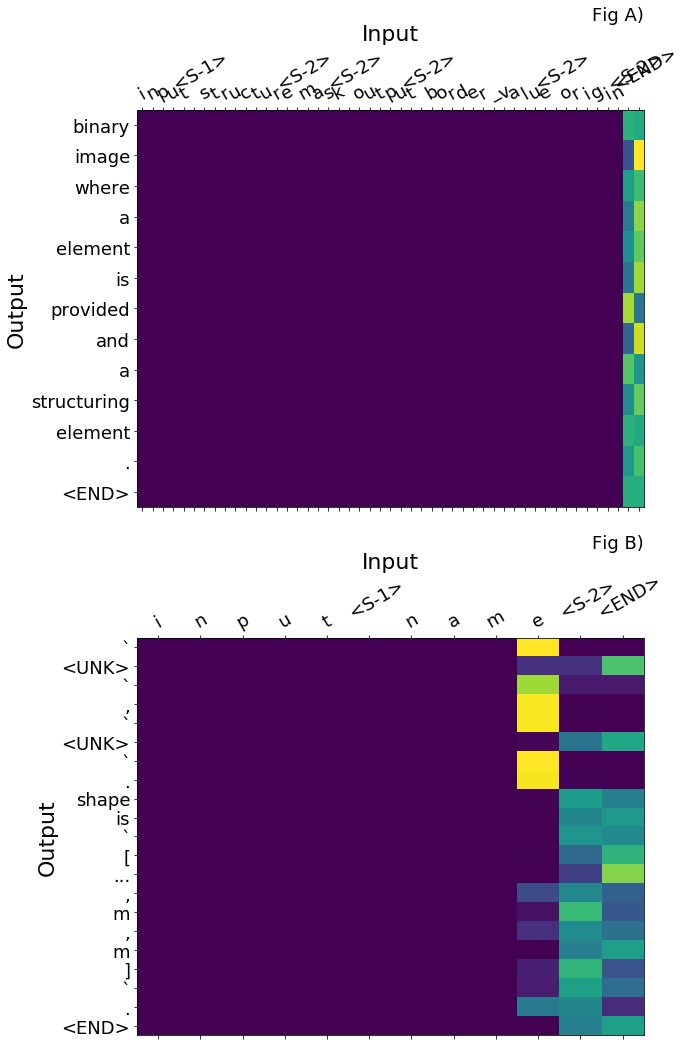
\includegraphics[width=0.7\linewidth]{images/otherargs_example.png}
    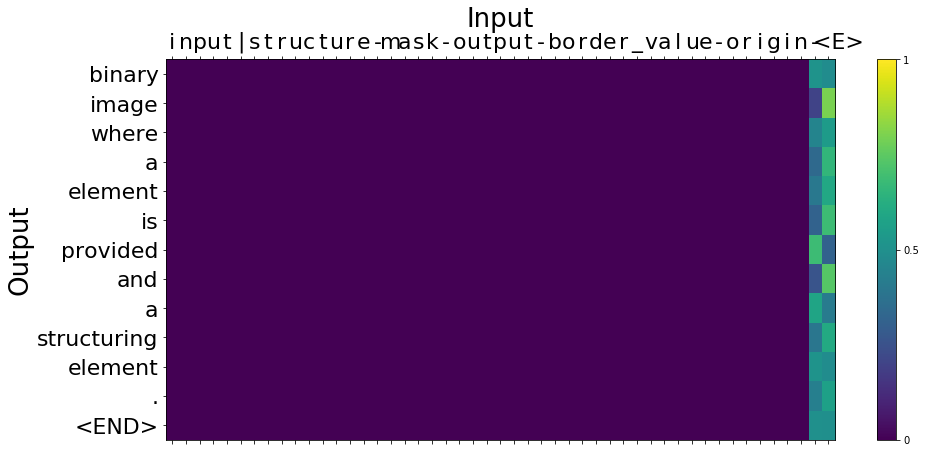
\includegraphics[width=0.9\linewidth]{ImagesCodeRelated/attn1pretty.png}
    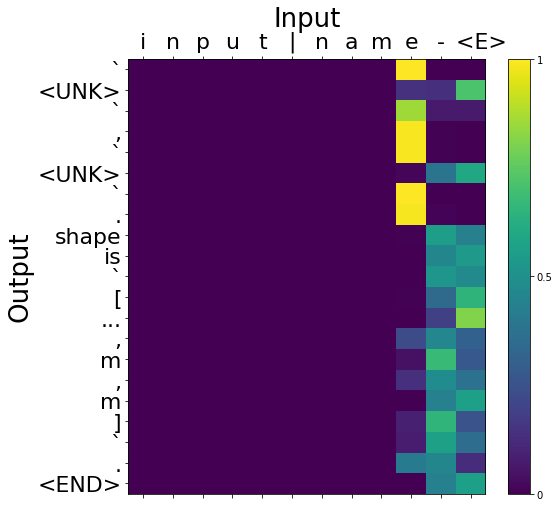
\includegraphics[width=0.5\linewidth]{ImagesCodeRelated/attn2pretty.png}
    \caption{An example of some the attentions of from the Name + Other Arguments tokenization on a Seq-to-Seq model, on the Reduced Random-Split Dataset. Fig A) is a picture of a typical example, Fig B) bottom is an example that is very overdetermined.}
    \label{fig:otherarg_attn}
\end{center}
\end{figure}

This implies the model is using all the extra information to encode a single vector to contextualise on, rather than learning to apply parts of the sequence to parts of translation, in an alignment fashion.
This single contextual vector can contain all the sequence information because the encoded RNN outputs at N can contain information from the previous N-1 tokens, and this in principle allows the model the condition word generation on the all the information up to the `attended' input token. 

Although this behaviour was expected for short sequences like variable names, we expected longer sequences (of up to 120 tokens) to be harder to compress, and suspected overcapacity of the LSTM might allow this learning strategy to take place. 
With less capacity, perhaps the final output of the RNN would not be as informative, instead relying on outputs at different points of the sequence
However, repeating the experiment with an LSTM encoder size of 75 resulted in the same pattern of attention, though with a much reduced BLEU score.

We also repeated the experiment on the much larger Full Random-Split dataset, where now just the input argument name would be certainly be the most important feature, due to repetitions points with the same name with the same description, but different co-arguments and function names. 
In this case we saw the final heavy attention shift to the separator just after the variable name - indicating that the model was learning where the most informative section of the data was, but was still choosing the encoded vector at that point. 
Interestingly we found that model did still take into account the rest of the sequence after this point (generating different translations), but that these all varied along a the same theme of the variable name. 
The attentions for a single example are given in Figure ~\ref{fig:otherarg_attn_full_dataset}

\begin{figure}

\begin{center}
    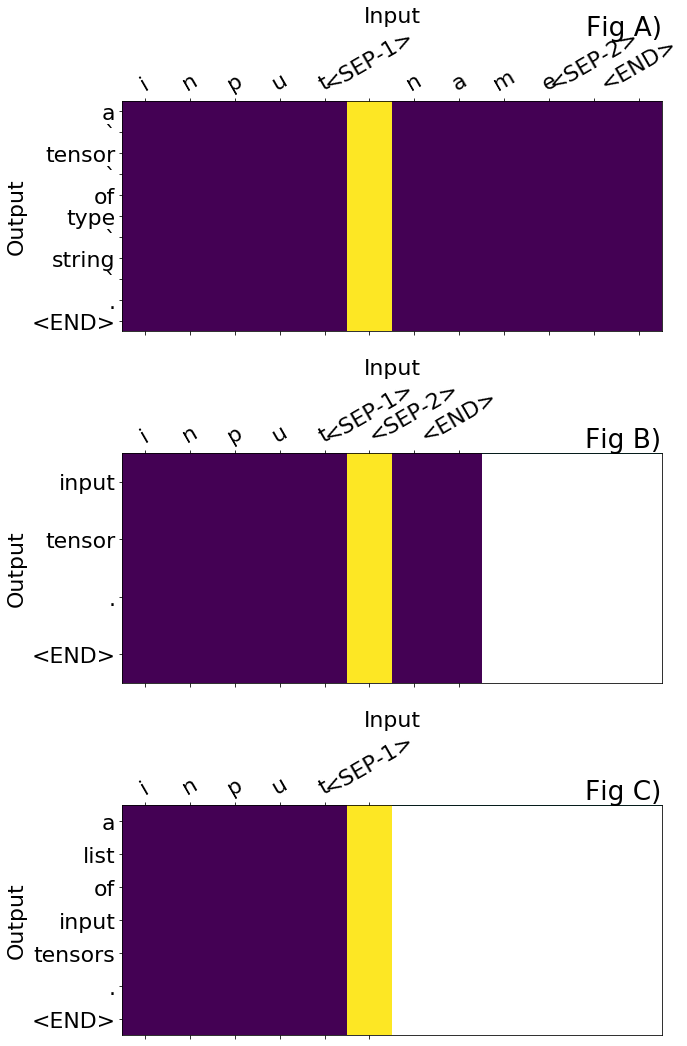
\includegraphics[width=0.7\linewidth]{images/different_translations_dupsXotherargs_3230minib_white.png}
    \caption{Three translations and attentions for an example of some the attentions of from the Name + Other Arguments on the tokenization on a Seq-to-Seq model trained on the Full Random-Split Dataset. Here is shows that, on the Full Random-Split Dataset, the most important feature is variable name, and the model attends solely to that, but that the hidden state of the LSTM still takes into account characters after the variable input }
    \label{fig:otherarg_attn_full_dataset}
\end{center}
\end{figure}

The conclusion to be drawn from this investigation is that the attention does not distribute well over characters, and these tokenizations actually behave much like longer single names, rather than features that can be distiguished separately. 
This leads to overfitting in many cases, as the some names are closer to unique, and you get a model that fits more like a Rote Learner. 
The model seems to work at its best when synthesising information as much as possible, but this seems more difficult to do when so much identifying information is given without information on redundancy. 
To give an example, Table \ref{table:example_plausible_training} shows the `plausible' example given above, with all training instances that start \mintinline[]{yaml}{input<SEP-1>structure}, highlighting that certain features of the final description are in the training ("binary image"), yet the potentially helpful sequence \mintinline[]{yaml}{<SEP-1>mask<SEP-1>} is ignored.

To counter this beahaviour in future, more work could be done both by investigating tokenizations or attention mechanisms.
In particular, the peaky nature of the softmax in attention could be replaced with a broader distribution, or the entropy of the softmax could be changed with a temperature parameter throughout training, to force the model to consider different sections of the data.
Ideally, combined with this differnet annention arrangement, more data would be provided that could help present a nuance to the arguments, rather than them simply being specifying information. 
Future work should at least investigate whether data augmentation by providing duplicates with arguments in different orders, perhaps also with synonyms of descriptions, could help models learn more generalisable descriptions.


\begin{table}
\begin{center}
\makebox[\linewidth][c]{
\begin{tabular}{l}

\hline
\textbf{Validation Example}\\

\textbf{I}: \mintinline[]{python}{i n p u t <SEP-1> s t r u c t u r e <SEP-2> m a s k <SEP-2> o u t p}...\\
...\mintinline[]{python}{u t <SEP-2> b o r d e r _ v a l u e <SEP-2> o r i g i n <SEP-2> <END>}\\
\textbf{D}: binary image to be propagated inside ` mask ` .\\
\textbf{P}: binary image where a element is provided and a structuring element . $<$END$>$\\
\\\hline\\

\textbf{Training Examples} starting \mintinline[]{yaml}{i n p u t <SEP-1> s t r u c t u r e}\\
\textbf{I}: \mintinline[]{yaml}{i n p u t <SEP-1> s t r u c t u r e 1 <SEP-2> s t r u c t u r}...\\
...\mintinline[]{yaml}{e 2 <SEP-2> o u t p u t <SEP-2> o r i g i n 1 <SEP-2> o r i g i n 2 <SEP-2> <END>}\\
\textbf{D}: binary image where a pattern is to be detected .\\
\\
\textbf{I}: \mintinline[]{yaml}{i n p u t <SEP-1> s t r u c t u r e <SEP-2> i t e r a t i o n s <SEP-2> o u t }...\\
...\mintinline[]{yaml}{p u t <SEP-2> o r i g i n <SEP-2> m a s k <SEP-2> b o r d e r _ v a l u e }\\
...\mintinline[]{yaml}{<SEP-2> b r u t e _ f o r c e <SEP-2> <END>}\\
\textbf{D}: binary array\_like to be closed . non-zero ( true ) elements form the subset to be closed .\\
\\
\textbf{I}: \mintinline[]{yaml}{i n p u t <SEP-1> s t r u c t u r e <SEP-2> o u t p u t <SEP-2> o r}...\\
...\mintinline[]{yaml}{i g i n <SEP-2> <END>}\\
\textbf{D}: n-dimensional binary array with holes to be filled\\
\\
\textbf{I}: \mintinline[]{yaml}{i n p u t <SEP-1> s t r u c t u r e <SEP-2> o u t p u t <SEP-2> <END>}\\
\textbf{D}: an array-like object to be labeled . any non-zero values in ` input ` are counted as features...\\
...and zero values are considered the background .\\
\\
\textbf{I}: \mintinline[]{yaml}{i n p u t <SEP-1> s t r u c t u r e <SEP-2> i t e r a t i o n s <SEP-2> m a s k }...\\
...\mintinline[]{yaml}{<SEP-2> o u t p u t <SEP-2> b o r d e r _ v a l u e <SEP-2> o r i g i n <SEP-2>}\\
...\mintinline[]{yaml}{b r u t e _ f o r c e <SEP-2> <END>}\\
\textbf{D}: binary image to be eroded . non-zero ( true ) elements form the subset to be eroded .\\
\\
\textbf{I}: \mintinline[]{yaml}{i n p u t <SEP-1> s t r u c t u r e <SEP-2> i t e r a t i o n s <SEP-2> m a s k}...\\
...\mintinline[]{yaml}{<SEP-2> o u t p u t <SEP-2> b o r d e r _ v a l u e <SEP-2> o r i g i n <SEP-2>}\\
...\mintinline[]{yaml}{b r u t e _ f o r c e <SEP-2> <END>}\\
\textbf{D}: binary array\_like to be dilated . non-zero ( true ) elements form the subset to be dilated .\\
\\



\end{tabular}
}
\caption{A validation example and the a selection of training points. Despite being a long sequence, }
\label{table:example_plausible_training}
\end{center}
\end{table}

%%% EXTRA PLOTS: Avergae attention over words
%%%.             Attention/Results of words shuffled



% What is the problem? Attention softmax is narrow and doesnt distribute well over characters, since there isn't really a one to one alignment. Instead what we see is the same behaviour as a much longer function name, where it works best when interpolating data. then give the plausibility

% Future work: Attention softmax is too narrow. Try a higher entropy distribution for character model
% Try a learning schedule
% Rotate the order of words, (done)
% Also more data.


% \begin{enumerate}
%     % \item we expected words to help choose bits in overdetermined cases. attention distributed across multiple words
%     % \item however we get attention focused on last word.
%     % \item The rnn final state acts as a good contextual vector for generation, we get good performance improvements on decoding
%     % \item The sort bonus is explained, but no change with longer.
%     \item It is possible the attention is being pathological. It's such a good strategy, that it stays there, and stops looking elsewhere, the weight decays to zero
%     % \item To investigate we ran with low lstm, -> no change in behaviour (LSTM 75), still tries to encode
%     \item We then tried to investigate if the rest of the data is being used (use the full dataset, and found that)
%     \item in cases with still degeneracy, attention is confused it panics (see bluring at end - can only explore nearest by states)
%     \item Check out Rote learner vs LSTM for "name" again. is it interpolating, or being a bad lstm (fitting bits of it, that dont transfer.)
%     \item We also take a closer look at the failures and notice a specific pattern. note tha in some cases the model works well, and. Basically hypothesise the size of the data with lack of indentifyin ginformation leads to overfitting, rather than just variable name which works.
% \end{enumerate}


\section{Investigating the Computer Readable Channel} % (fold)
\label{sec:investigating_the_computer_channel}

\subsection{Comparing Code2Vec to Baselines} % (fold)
\label{sub:comparing_code2vec_to_baselines}


\subsubsection{Experiment Objective} % (fold)

In our first examination of the computer readable channel we aimbed to validate our initial hypothesis that simply the code could be informative when predicting argument descriptions.
In particular we wished to assess what possible tokenizations of code paths from the syntax tree could prove most informative, and set up as strong baseline as possible against which would compare our neural model.



\subsubsection{Method \& Results} % (fold)

For this experiment we used the Full Random-Split Dataset, to make the most of the different code paths associated with each argument.
We followed the vocabulary generation and source code tokenization procedures outlined in section X. 
We used a vocabulary size of 15000 for both path strings and terminal nodes, and set the maximum number of paths per argument to  5000.
These values were sought to be as large as possible for the size of the GPU. 

We then ran our Rote Learner, using the four different matching code path only criteria, outlined in section X. 
These chose a description from a set of training samples by:
    \begin{itemize}
        \item combining samples with largest subpath overlap for each path in test, and chosing from that list. (Sub Path Proportional)
        \item combining samples with largest subpath overlap for each path in test, and chosing from the most frequent training point(s) in that list. (Sub Path Max)
        \item combining samples full overlap for each path in test, and chosing from that list (Full Path Proportional)
        \item combining samples full overlap for each path in test, and chosing from the most frequent training point(s) in that list. (Full Path Max)
    \end{itemize}
Each of these was run 50 timesto overcome the stochasticity of the Rote Learner.

We then ran the Code2Vec Decoder, following the usual training procedure, for a maximum of 100 epochs.
We selected the model with the best BLEU score in that time.
The hyperparameters for this model are found in Table {X}.

We report our results in Table \ref{table:name_code2vec_solo}, noting that the Rote Learner performed best using the Full Path Max matching, with a BLEU score $ 11.82 \pm  0.16 $ and  $ 12.61 \pm 0.12 $ on validation and test, but that the Code2Vec Decoder significantly outperformed this, achieving a BLEU score of $ 18.94 $ and $ 18.13 $ on validation and test respectively.

From the Rote Learning perspective, the next best criterion was the Sub Path Max, which achieved a corpus level BLEU score of $ 6.93 \pm  0.34 $ and $ 7.09 \pm 0.22 $ on validation and test respectively.  
The two remaining Proportional criteria performed worst, each about 6 bleu points worse than their counterparts

These results confirmed that looking at code paths would indeed be informative, and indicated that investigating full codepaths would indeed be the best way to start. 
They also showed great promise for the Code2Vec Decoder as a model.

% subsection comparing_code2vec_to_baselines (end)

\begin{table}[ht!]
\begin{center}
\begin{tabular}{ c | c | c  }
    Model                             & BLEU Validation  & BLEU Test      \\
    \hline
    Rote Learner (codeonly)                  &  &  \\
    - \textit{Subpath Proportional}              & $ 0.71 \pm  0.13 $ & $ 0.74 \pm 0.07 $   \\
    - \textit{Subpath Max}                       & $ 6.93 \pm  0.34 $ & $ 7.09 \pm 0.22 $  \\
    - \textit{Full Path Proportional}            & $ 4.94 \pm  0.28 $ & $ 5.11 \pm 0.18 $  \\
    - \textit{Full Path Max}                     & $ 11.82 \pm  0.16 $ & $ 12.61 \pm 0.12 $  \\
    \hline
    Code2Vec Decoder                             & $ 18.94 $ & $ 18.13 $  \\
    % \hdashline
    % Code2Vec                          & $ 12.64199 $ & $ 12.80257 $  \\
    \hline 
    % Model                             & BLEU Validaion  & BLEU (Test)      \\
    % \hline
    % Rote Learner (codeonly)           &  & & \\
    % - \textit{softest}                     & $ 0.70702 \pm  0.13979 $ & $ 0.73623 \pm 0.07094 $   \\
    % - \textit{soft}                        & $ 6.93465 \pm  0.33987 $ & $ 7.09349 \pm 0.21836 $  \\
    % - \textit{hard}                        & $ 4.94109 \pm  0.28153 $ & $ 5.11432 \pm 0.18345 $  \\
    % - \textit{hardest}                     & $ 11.82453 \pm  0.15695 $ & $ 12.61319 \pm 0.12093 $  \\
    % \hline
    % Code2Vec   !!                            & $ 18.93630 $ & $ 18.12909 $  \\
    % % \hdashline
    % % Code2Vec                          & $ 12.64199 $ & $ 12.80257 $ & \\
    % \hline
\end{tabular}
\caption {BLEU Scores on the Full Random-Split Dataset, for Code2Vec Decoder and a series of code only Rote Learners}
\label{table:name_code2vec_solo}
\end{center}
\end{table}

\subsubsection{Analysis} % (fold)
\label{ssub:analysis}

In order to investigate the behaviour of the Code2Vec model, we sampled points from the validation set, printed out the source code, paths and attentions as they passed through the model.
We observed that sometimes the model overfit some particular paths, with very high attentions on a single point, but more often than not the model distributed its attention over 4 or 5 paths, even if there were thousands to choose from.

A single example of such an analysis, where multiple paths are attended and the different paths are easy to see, is presented in Figure  \ref{fig:single_examples} .
It shows the pretokenized syntax tree, the attented paths, the source and the translation.
From this example it is interesting to note that the model has chosen two paths that indicate list comprehensions feature in the variable, and it has inferred that a list should feature in the description from the code alone.

Noting that the model seemed to be performing as expected on a microscopic level, we continued to investigate the behaviour of the model across the entire validation set. 
Figure \ref{fig:entropy_code2vec} shows a the distribution of the entropies of the attentions of the Code2Vec vectors, for each point in the validation set. 
Presented along side, is the distribution of entropies that would have occured if every data point in the validation set had attained a uniform, categorical distribution as attention.
The shift to a lower entropy clearly verifies that the Code2Vecs attention focuses on only a fraction of the paths, and, in some few cases (where the entropy is effectively 0) decides resolutely on single points.

Figure \ref{fig:sentence_bleu} shows the counts of sentence level BLEU score of each sentence in the validation set.
Although this metric is prone to low scores on individual sentences <CITE> over the whole corpus, we can use it to get a sense for where the performance improvements come from in the Code2Vec Model.
From this graph it is one can see both a significant increase in the models 1.0 scoring sentences, and also a modest increase in low scoring sentences. 
This indicates both an improvement that may be down to some form of overfitting (the model is able to find arguments that are very similar, and have similar code paths), but also an improvement due to generating just a few of the correct words, as in the example presented above. 


\begin{table}[ht!]
\begin{center}

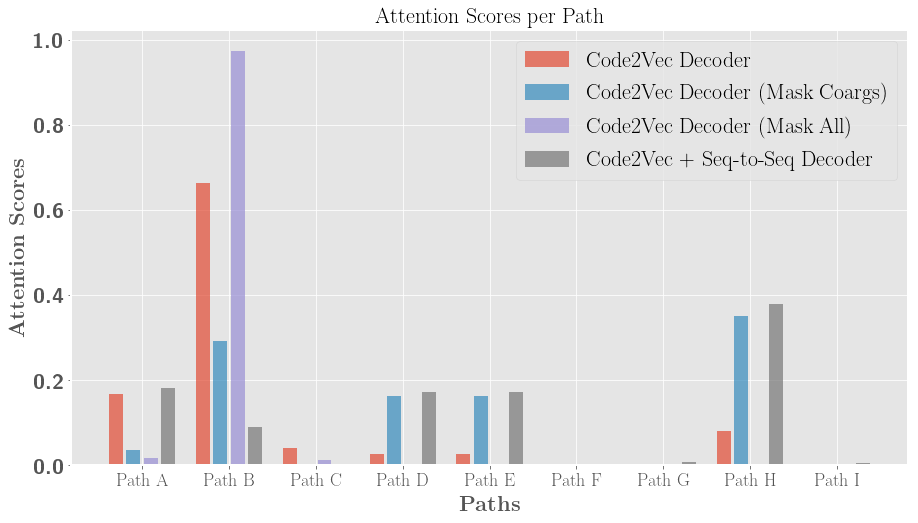
\includegraphics[width=0.9\linewidth]{ImagesCodeRelated/pretty_attention_XKCD.png}
        % how to set font size here to 10 px ?  
\begingroup
    \fontsize{10pt}{12pt}\selectfont
\begin{tabular}{c l}
    & \textbf{Paths} \\
    \\
    \textbf{Path A} & Name $\leftarrow$ comprehension $\leftarrow$ ListComp $\leftarrow$ Assign $\rightarrow$ Name : \mintinline[]{yaml}{palette} \\
    \textbf{Path B} & Name $\leftarrow$ comprehension $\leftarrow$ ListComp $\rightarrow$ comprehension : \mintinline[]{yaml}{<UNK>} \\
    \textbf{Path C} & $<$UNK$>$ : \mintinline[]{yaml}{color_palette} \\
    \textbf{Path D} & Name $\leftarrow$ comprehension $\rightarrow$ Name : \mintinline[]{yaml}{name} \\
    \textbf{Path E} & $<$UNK$>$ : \mintinline[]{yaml}{palette} \\
    \textbf{Path F} & $<$UNK$>$ : \mintinline[]{yaml}{palette} \\
    \textbf{Path G} & $<$UNK$>$ : \mintinline[]{yaml}{len} \\
    \textbf{Path H} & $<$UNK$>$ : \mintinline[]{yaml}{name} \\
    \textbf{Path I} & $<$UNK$>$ : \mintinline[]{yaml}{<UNK>} \\
\end{tabular}
\endgroup

% \caption{Example Attention Scores}
% \end{table}

\end{center}
\caption{Code \& List}
\label{fig:single_examples}
\end{table}


\begin{figure}
\begin{center}
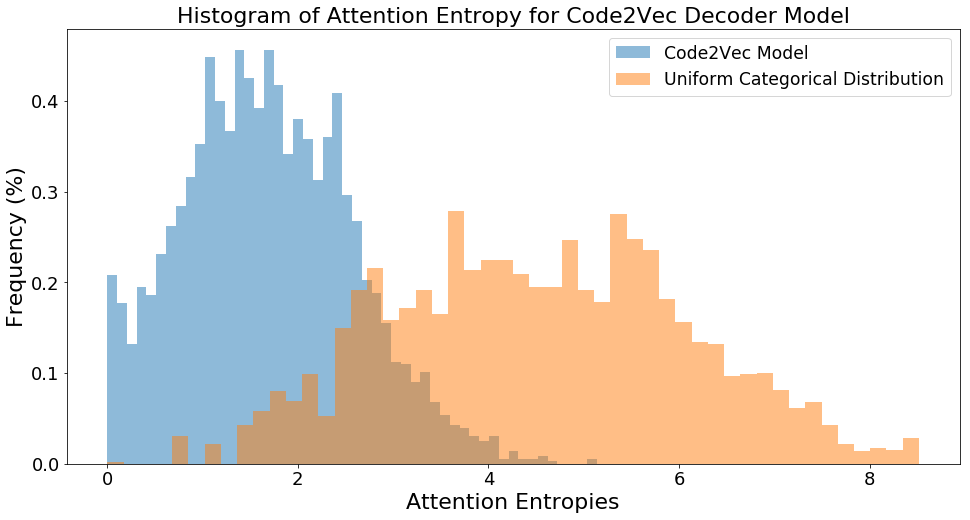
\includegraphics[width=0.8\linewidth]{ImagesCodeRelated/code2vec_entropies.png}
\end{center}
\caption{code2vec entropy}
\label{fig:entropy_code2vec}
\end{figure}


% \begin{enumerate}
%     \item With the code lstm we see some of the behaviour we like, but also, only overfitting. There is no sequence so in some cases, a path or a single variable can be informative, but it performs well.
%     \item See a single example and distribution of attention.
%     \item CLearly there are a lot of spikes compared to uniform. More masking the more spiking, though this is partly due to best bleu. Compare at cross entropy time?
%     \item Then look at, bleu per sentence, maybe av bleu per sentence per attn entropy.
%     \item Big COMPARE vs ROTE LEARNER - can we conclude this is worth more researcg?
%     \item Cna show how choices change w model for given example??

%     \item C2VEnc: does combining add anythin? More capacity, check weights.
% \end{enumerate}

% \begin{table}


% subsubsection analysis (end)

\subsection{Masking Identifiers in Code2Vec} % (fold)
\label{sub:comparing_code2vec_altered}

\subsubsection{Experiment Objective} % (fold)

The Code2Vec Decoder model uses a vocabulary of terminal nodes to generate code paths. 
Due to the python abstract syntax tree, these are almost always names, which could be either those of internal variables, built-in functions or even out of scope objects. 
We investigated masking these terminal node names, to be conclude that that the structure of the code was providing a valuable signal to the Code2Vec Decoder, beyond the ideosyncracies of variable and method naming.

\subsubsection{Method \& Results} % (fold)

We used the same dataset and tokenization procedure as described in Section \ref{sub:comparing_code2vec_to_baselines} to prepare the tokenized code paths as before.
However, this time we investigated two different masking procedures, to hide the terminal node from the models.

In the first masking, we masked the only the coarguments in the code paths.
We did this by creating new terminal node identifiers, for "first coargument", "second coargument", and so forth, and renaming all terminal node identifier indices to these numbers.
This means that the model can still recognise when two code paths belong to the same terminal node, but no embedding can be generated linking the fact that that argument shares a coargument name with any other variables.

In our second masking, we masking we repeated this procedure, but for every point in the dataset.
This meant that very indicative global variables were masked, but also any inbuilt method.
Instead the model only had access to enough information to be able to differentiate terminal nodes within a function.

Once again we trained these for 100 epochs, with the hyperparameters specified in Appendix X.

We present the results in Table \ref{table:code_2_vec_masked}, noting that Coargument Masking only resulted in a slight performance drop, of one to two BLEU points, from the unmasked variables, while the Full Masking resulted in a significant drop of six BLEU points, while still beating the best Rote Learner baseline.



\begin{table}[ht!]
\begin{center}
\begin{tabular}{ c | c | c }
    Model                             & BLEU (Unsplit)  & BLEU (Split)    \\
    \hline
    Rote Learner (best performer)          & $ 11.82453 \pm  0.15695 $ & $ 12.61319 \pm 0.12093 $ \\
    \hline
    Code2Vec                               & $ 18.93630 $ & $ 18.12909 $ \\
    Code2Vec  (Coargument Masking)              & $ 17.01868 $ & $ 16.93701 $ \\                  
    Code2Vec  (Full Masking)                & $ 13.27677 $ & $ 13.07374 $ \\
    % \hdashline

    % Code2Vec                              & $ 12.64199 $ & $ 12.80257 $ & \\
    % Code2Vec (masked args)                & $ 12.10462 $ & $ 11.93314 $ & \\
    % Code2Vec (masked all)                 & $ 9.01463 $ & $ 9.15697 $ & \\
    \hline
\end{tabular}
\caption {Investigate code2vec but with masked variables}
\label{table:code_2_vec_masked}
\end{center}
\end{table}


\begin{figure}
\begin{center}
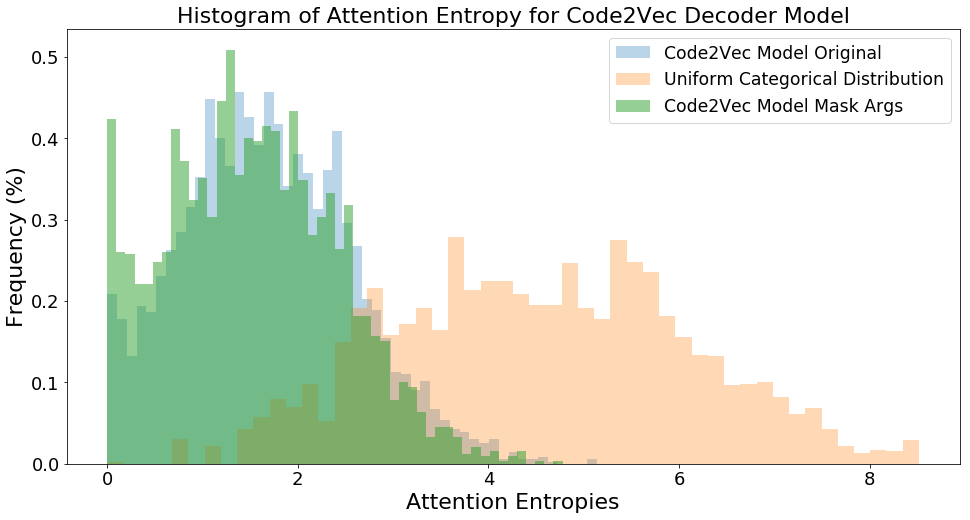
\includegraphics[width=0.8\linewidth]{ImagesCodeRelated/entropies_mask_args.png} 
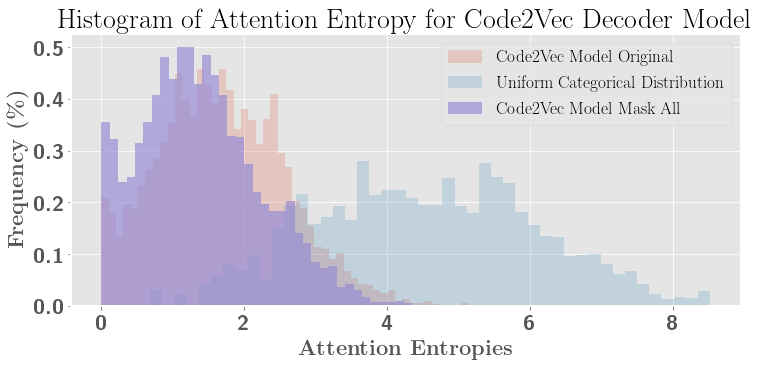
\includegraphics[width=0.8\linewidth]{ImagesCodeRelated/entropies_mask_all.png}
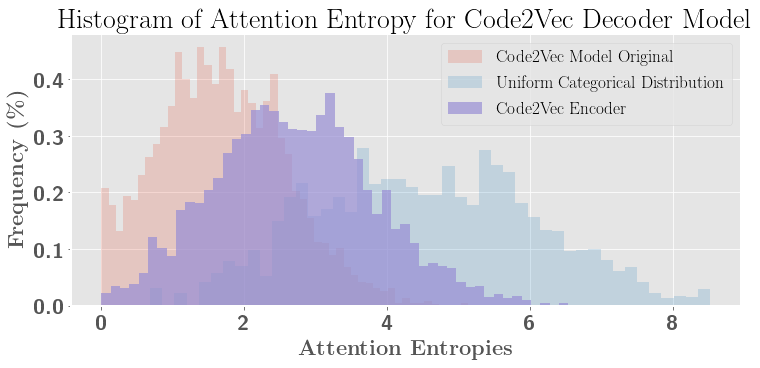
\includegraphics[width=0.8\linewidth]{ImagesCodeRelated/entropies_encoder.png}
\end{center}
\caption{all entropies}
\label{fig:all_entropies}
\end{figure}


\subsubsection{Analysis} % (fold)

Once again we investigated the performance of these models on the validation set, examining the entropies of both the masked models, on the validation dataset.

Noting the BLEU score and the lack of shift of the center of the entropies, it appears that losing coarguments, when the rest of the code is present, does not significantly impact the models behaviour.
There is a spike in the number of attentions with close to zero entropy, which could be explained by having informative codepaths involving coarguments, now being accessed more regularly at test time, but otherwise there is little change.

However, for the fully masked arguments we see alarge shift to even lower entropys, and greater mass closer to 0 entropy. In these cases it is likely the model is simply fitting to the paths it recognises, as the target nodes become less informative, and we start to see a performance of the model that starts to come close to the Rote Learner.

However, this experiment shows that by completely renaming all variables (including aliasing built-ins!), the model is still able to learn features from the paths of the source code themselves, suggesting that types of variables, and idiomatic expressions can add information, even in potentially very large syntax trees.


\begin{figure}
\begin{center}
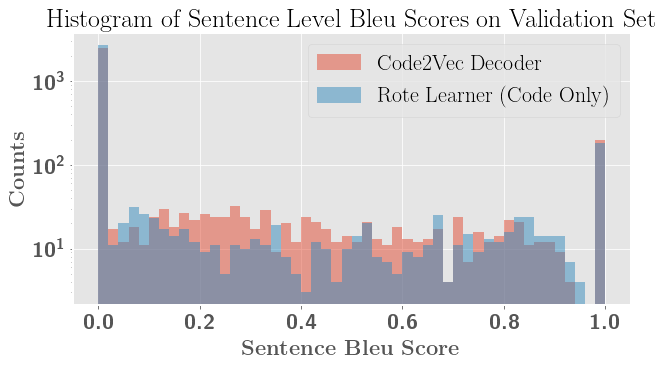
\includegraphics[width=0.75\linewidth]{ImagesCodeRelated/pretty_sentence_c2v.png}
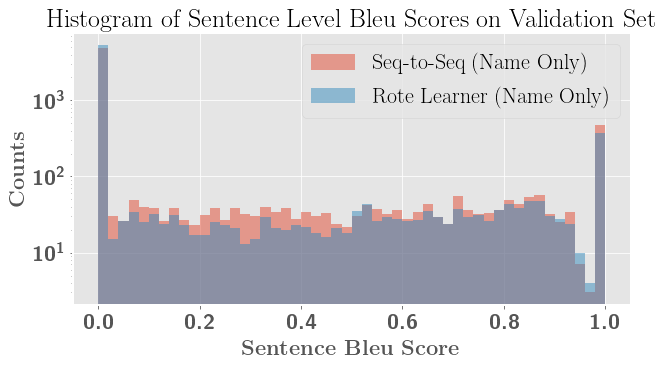
\includegraphics[width=.75\linewidth]{ImagesCodeRelated/pretty_sentence_bleu_s2s.png}
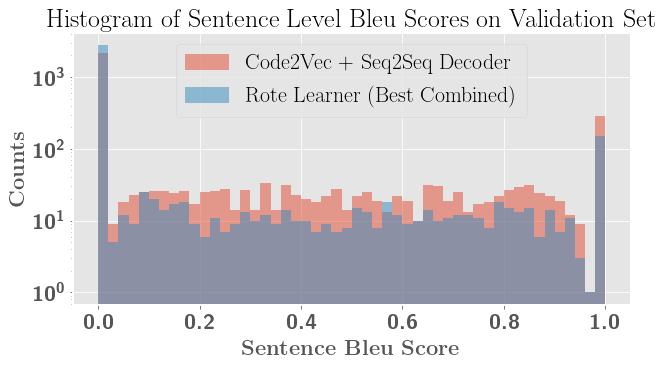
\includegraphics[width=.75\linewidth]{ImagesCodeRelated/pretty_sentence_bleu_c2e.png}
\end{center}
\caption{sentence bleu}
\label{fig:sentence_bleu}

\end{figure}

\begin{listing}[h!] 
\begin{center}

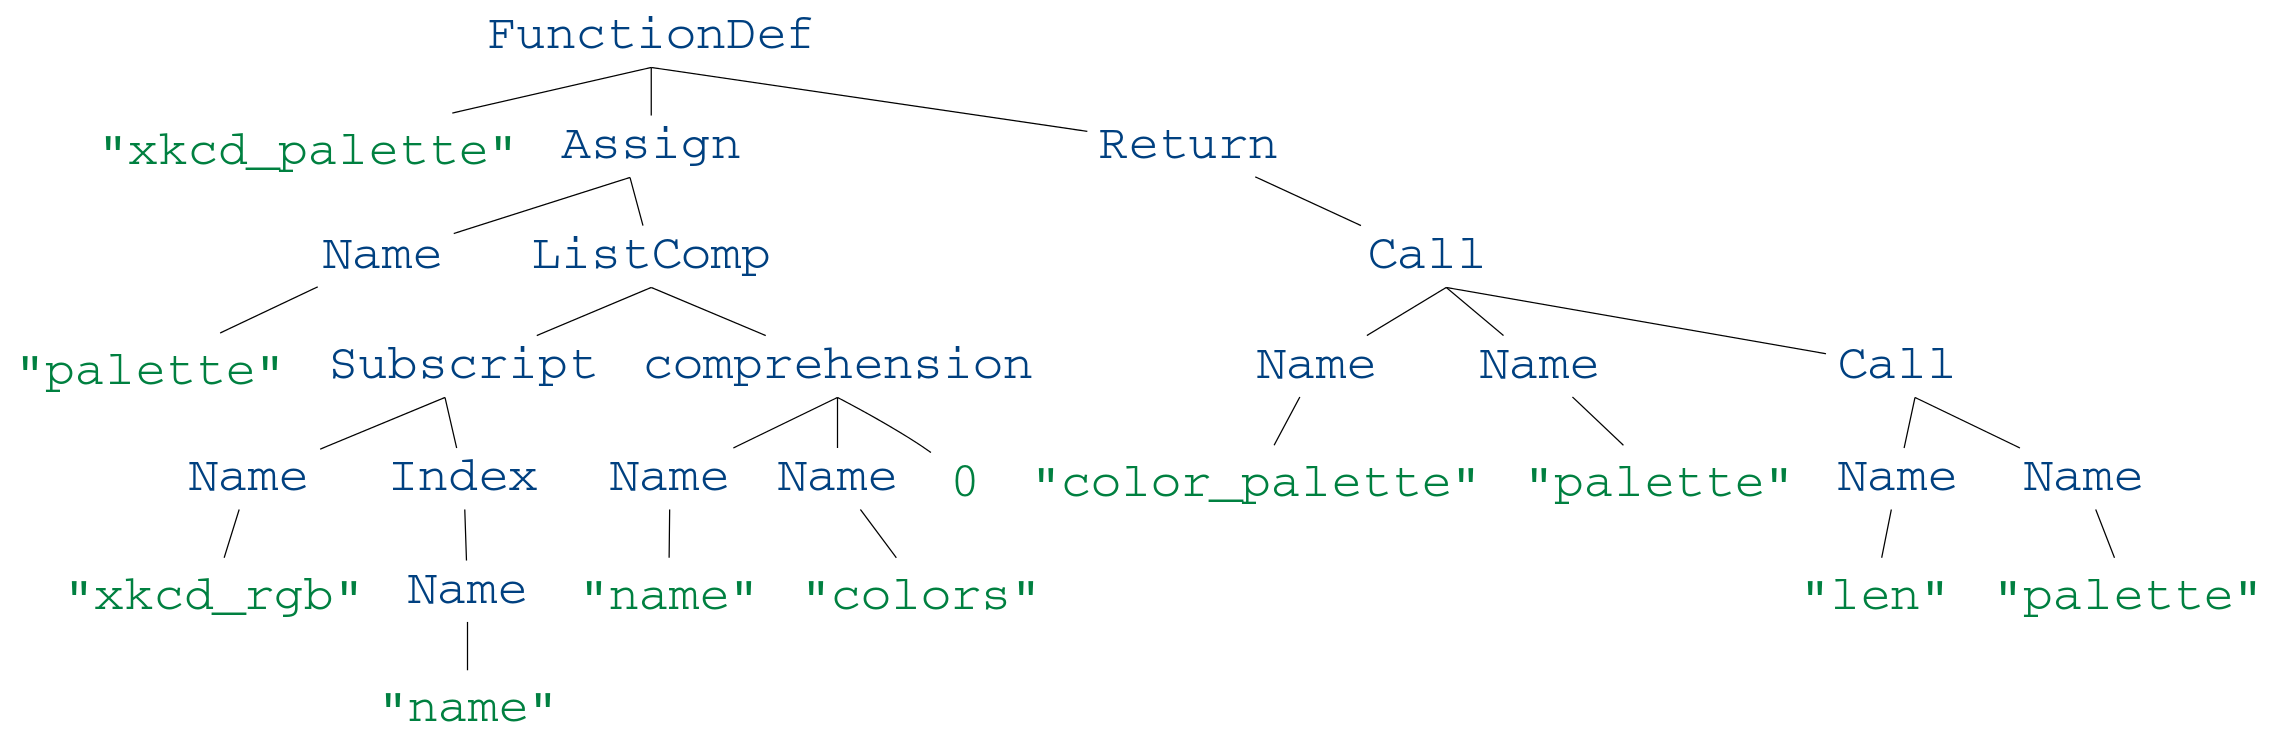
\includegraphics[width=\linewidth]{ImagesCodeRelated/xkcd_palette_strip.png}
\begin{minted}[]{python}
def xkcd_palette(colors):
    palette = [xkcd_rgb[name] for name in colors]
    return color_palette(palette, len(palette))

\end{minted}
\begin{tabular}{l}
\textbf{I}: \mintinline[]{python}{colors}\\
\textbf{D}: list of keys in the `` seaborn.xkcd\_rgb `` dictionary .\\
\textbf{P}: a list of data to read . if none , all other the first will be returned .\\
\end{tabular}
\end{center}
\end{listing}







\section{Investigating Combined Channels} % (fold)
\label{sec:investigating_combined_channels}


\subsection{Combined Code2Vec } % (fold)
\label{sub:combined_code2vec}

% subsection comparing_code2vec_to_baselines (end)

\subsubsection{Experiment Objective} % (fold)

Both the Seq-to-Seq models and Code2Vec Decoder models fundamentally look at different modalities of code when making their inference.
In this investigation we sought to investigate what could happen by combining these two modalities of information in the Code2Vec + Seq2Seq Decoder.

\subsubsection{Method \& Results} % (fold)

Given the nature of the code elements of this investigation, we continued with the Full Random-Split Library, and proceeded with the same format of investigation as outlined in previous sections. 
We ran the full neural models for 100 epochs, using the name only tokenizations for the human readable channel and the full unmasked paths for the code2vec encoder.

The results of these experiments are presented in Table \ref{table:code2vec_embed}. 
We report that the combined model surpasses both individual models achieving a BLEU of $28.7$ and $27.08$ on validation and test respectively. 
However, this is only making a small improvement on the Seq-to-Seq models, of about 2 points. 
This is at least partly down to the presence of (name, description) duplicate pairs in the dataset, which boosts both the performance of the Seq-to-Seq, and that of the rote learner.

It is interesting to note that the combined Rote Learner model performs worse when trying to learn on both modalities, achieving a score of $15.0$ annd $15.75$, which underperforms the name only model of $19.0$ and $19.68$ on validation and test.  


\begin{table}[h!]
\begin{center}
\begin{tabular}{ c | c | c  }
    Model                             & BLEU Validation  & BLEU Split     \\
    \hline
    Rote Learner  (code only)        & $ 11.84 \pm  0.16 $ & $ 12.62 \pm 0.12 $ \\
    Code2Vec Decoder                 & $ 18.94 $ & $ 18.13 $ \\
    % \hdashline
    % Code2Vec  (code only)             & $ 12.64199 $ & $ 12.80257 $ & \\
    \hline
    \hline
    Rote Learner  (name only)         & $ 19.04 \pm  0.35 $ & $ 19.69 \pm 0.28 $ \\
    Seq2Seq (name only)               & $ 26.40 $ & $ 25.40 $ \\
    % \hdashline
    % Seq2Seq  (name only)              & $ 15.94701 $ & $ 15.71091 $ & \\
    \hline
    \hline
    Rote Learner (combined)            & $ 15.02 \pm  0.45 $ & $ 15.76 \pm 0.30$ \\
    Code2Vec+ Seq-to-Seq Decoder       & $ 28.77 $ & $ 27.68 $ \\
    % \hdashline
    % Code2Vec  + Char to Seq           & $ 23.11775 $ & $ 22.37520 $ & \\
    % \hline
    % Model                             & BLEU Validation  & BLEU Split     \\
    % \hline
    % Rote Learner  (code only)        & $ 11.83875 \pm  0.15697 $ & $ 12.62479 \pm 0.12103 $ \\
    % Code2Vec Decoder                 & $ 18.93630 $ & $ 18.12909 $ \\
    % % \hdashline
    % % Code2Vec  (code only)             & $ 12.64199 $ & $ 12.80257 $ & \\
    % \hline
    % \hline
    % Rote Learner  (name only)         & $ 19.03534 \pm  0.35183 $ & $ 19.68826 \pm 0.28100 $ \\
    % Seq2Seq (name only)               & $ 26.39189 $ & $ 25.39841 $ \\
    % % \hdashline
    % % Seq2Seq  (name only)              & $ 15.94701 $ & $ 15.71091 $ & \\
    % \hline
    % \hline
    % Rote Learner (combined)            & $ 15.01764 \pm  0.44897 $ & $ 15.75528 \pm 0.29560 $ \\
    % Code2Vec+ Seq-to-Seq Decoder       & $ 28.76581 $ & $ 27.68100 $ \\
    % \hdashline
    % Code2Vec  + Char to Seq           & $ 23.11775 $ & $ 22.37520 $ & \\
    \hline
\end{tabular}
\caption {Investigate code2vec combined with seq to seq}
\label{table:code2vec_embed}
\end{center}
\end{table}

\subsubsection{Analysis} % (fold)


Analysis of the combined models largely followed the pattern of those in sections \ref{sec:investigating_the_computer_channel}, which involved looking at the entropies of the Code2Vec attention distributions and the sentence level BLEU scores, as evaluated over the whole of the validation set.

We found the unsurprisingly the Code2Vec + Seq to Seq Decoder model has a significantly wider distribution of entropies, centered around a higher point. 
This may partly be down to the fact that the model is now also learning from the highly informative variable name, and so depends less heavily on the specific code2vec paths. Nonetheless it still indicates the model is paying attention the codepaths when it makes its decisions.

This indicates why the model should outperform the Seq-to-Seq, but it given it is only a small improvement, it suggests that most of the performance gain comes from the name element of the data. 
Indeed, examining the distributions of sentence level BLEU scores, as visible in  \ref{fig:sentence_bleu}, suggests that te Seq-to-Seq model largely acts as a better Rote Learner, showing most of its improvements in the 1.0 scoring sentences. 
This is unsurprising given the number of duplicates of (name, description) pairs in this dataset.
Given the proximity of the BLEU scores for the Seq-to-Seq and Code2Vec + Seq-to-Seq scores, it is reasonable to assume a similar behavious is also occuring to some degree in the combined model.

% This is in agreement with the distribution of bleu scores in \ref{fig:sentence_bleu} v 

%  it is clear the availability of (name, description) duplicates helps both the name only learners, outperform the code only models ands suggests why the name only Rote Learner out performs the combined model. 

\section{Investigating the Library Split Dataset} % (fold)
\label{sec:analysis}

\subsubsection{Experiment Objective} % (fold)

Our final investigation sought to apply the most difficult test to our models, namely to investigate whether different modalities of code could help generate argument descriptions across completely differnet code bases and different authors.
This involved taking our strongest models and repeat them on our Full Library-Split Dataset.

\subsubsection{Method \& Results}  % (

The method of our investigations was as outlined above. In this case the models required significantly less training, plateauing their BLEU scores very early. We selected the best models that ran for at most 40 epochs. 
The results for each experiment is visible in Table \ref{table:split_datasets_embed}, with the hyperparameters presented in Table X.

We report that the neural model significantly struggled to learn the labelled translations on the library split datset.
The weakest models, the code only Code2Vec Decoders, scored BLEU scores of $0.89$ on both train and dev, very close to the code only Rote Learner score of   $ 1.01257 \pm  0.11410$, while the argument name models manage to achieve BLEU scores of about $1.5$ across both the Rote Learner and Seq-to-Seq models. 
Finally, the combined model of the Code2Dev + Seq-to-Seq model performs best, by a marginal amount, scoring  $ 1.85 $ and $ 1.59 $ across validation and test sets respectively,  outperforming the combined Rote Learner on both modalities byt about half a BLEU point.



\begin{table}[!ht]
\begin{center}
\begin{tabular}{ c | c | c }
    Model                             & BLEU Validation & BLEU Test \\
    \hline
    Rote Learner  (code only)         & $ 1.02 \pm  0.11 $ & $ 0.85 \pm 0.05 $ \\
    Code2Vec                          & $ 0.89 $ & $ 0.89 $ \\
    Code2Vec  (Mask Co-arguments)             & $ 0.67 $ & $ 0.67 $ \\
    Code2Vec  (Mask All)             & $ 0.69 $ & $ 0.71 $ \\
    \hline
    \hline
    Rote Learner  (name only)         & $ 1.44 \pm  0.17 $ & $ 1.36 \pm 0.06$ \\
    \hline
    Seq2Seq                             & &   \\
    - \textit{name only}              & $ 1.53 $ & $ 1.582$ \\
    - \textit{name + function name}      & $ 1.55 $ & $ 1.52 $ \\
    - \textit{name + co-argument names}         & $ 1.53 $ & $ 1.45$ \\   
    - \textit{name + function name +co-argument names}     & $ 1.51 $ & $ 1.48$ \\
    \hline
    \hline
    Rote Learner (combined)            & $ 1.23 \pm  0.169 $ & $ 1.157 \pm 0.101 $ \\
    Code2Vec  + Char to Seq            & $ 1.85 $ & $ 1.59 $ \\\\
    \hline


    % Model                             & BLEU Validation & BLEU Test \\
    % \hline
    % Rote Learner  (code only)         & $ 1.01257 \pm  0.11410 $ & $ 0.84707 \pm 0.04996 $ \\
    % Code2Vec                          & $ 0.88741 $ & $ 0.89466 $ \\
    % Code2Vec  (Mask Co-arguments)             & $ 0.66894 $ & $ 0.67366 $ \\
    % Code2Vec  (Mask All)             & $ 0.69457 $ & $ 0.71360 $ \\
    % \hline
    % \hline
    % Rote Learner  (name only)         & $ 1.43480 \pm  0.16744 $ & $ 1.36063 \pm 0.06452 $ \\
    % \hline
    % Seq2Seq                             & &   \\
    % - \textit{name only}              & $ 1.53474 $ & $ 1.58206 $ \\
    % - \textit{name + function name}      & $ 1.54843 $ & $ 1.52191 $ \\
    % - \textit{name + co-argument names}         & $ 1.53296 $ & $ 1.45225 $ \\   
    % - \textit{name + function name +co-argument names}     & $ 1.50983 $ & $ 1.48267 $ \\
    % \hline
    % \hline
    % Rote Learner (combined)            & $ 1.23201 \pm  0.16873 $ & $ 1.15672 \pm 0.10083 $ \\
    % Code2Vec  + Char to Seq            & $ 1.84887 $ & $ 1.58697 $ \\\\
    \hline
\end{tabular}
\caption {Investigate split datasets}
\label{table:split_datasets_embed}
\end{center}
\end{table}




\subsubsection{Analysis}

These results at first glance seem to indicate that the neural models can perform no better in generalised translation than the overfitting Rote Learner models.
However these low BLEU scores give little indication to the type of translations that are being generated.
To investigate the quality of these translations we examined a random sample of translations from both the Rote Learner and the Code2Vec models. 
A random sample are shown in Table \ref{tab:lib_split}.

In these we see very little overlap, though the translations make grammatical sense. 
In particular the types of descriptions generated appear shorter and more general than their counterparts with the Rote Learner, but both generally have a poor alignment with the true description.

% Although we see a very low ngram overlap,
% 1)  descriptions of the neural models seem plausible, and certainly less repeated and specific that Rote Learner.
% 2) (However,) looking at the one word overlap of the the models we see the following distributions.
% Searching for direct repeats of translations we find that X of the validation sentences are found in the training, indicating /not invdicating overfitting.

These low BLEU scores, despite grammatical sounding descriptions, lead us to the biggest problem with this task.
Generalisation across code documentation is difficult when code is written by different authors, with different contexts and conventions. 
Although related work in section X demonstrates that idioms and patterns in code do exist, we are fundamentally hampered by the both the variance of code between libraries and variation of the target language that we aim to generate when we split between libraries.
Codebases develop idioms and name conventions within libraries, and often have a context when it comes the language used in descriptions. 
Unlike in many words in the real world, descriptions of code artefacts are almost always metaphorical (for instance "colours", instead of "list of strings"),  and therefire different libraries are under no obligation to use the same language, or even vocabularies when referring to the same underlying code objects. 

For instance a list of strings could just as easily by a \mintinline[]{python}{x_axis_labels} or \mintinline[]{python}{song_categories}, but generating language surround the second example may be difficult without training examples without example of the relevant context.
 In the abstract the model may be able to infer something general, such as the type, but again idiomatic use of the code would need to be provided for this.

This lack of context and vocabulary, both with code and text, seems to be the case with our datasets.
We investigated how the different train set and validation set description vocabularies varied between the Random-Split and Library-Split Datasets after tokenization, and found that the in our Library Split dataset, the vocabularies of our training set are reduced by over 10\%, compared to a Random Split. 
Furthermore, we also found that after tokenization 16\% of the words in our validation set vocabulary do not even appar in the training set - even though these are not "UNK" tokens. This is almost a fourfold increase compared to the Random Split dataset.

\begin{table}
    \begin{center}
        \begin{tabular}{c c c}
           \hline
            & Random Split & Library Split \\
            \hline
            Tokenized Train Description Vocab Size    & 5249  &  4701 \\
            Tokenize Valid Description Vocab Size    & 3012  &  2866 \\
            \% of Tok. Valid Vocab not in Tok. Train Vocab                & 4.1\% &  15.8\% \\
            \hline
            \% of $<$UNK$>$ path elements in Train          &  37.4\%  &  32.4 \%   \\
            \% of $<$UNK$>$ path elements in Validation     &  37.5\%  &  57.4\% \\
            \% of $<$UNK$>$ terminal nodes in Train         &  12.3\%  &  8.8\%  \\ 
            \% of $<$UNK$>$ terminal nodes in Validation    &  14.7\% &  44.9\% \\   
            \hline
        \end{tabular}
    \end{center}
    \caption{A table showing the change in the actual vocabulary of the argument descriptions, and also change in out-of-vocabulary tokens, for different library splits.}
    \label{tab:vocabsplit}
\end{table}



This behaviour is even worse when it comes to the code paths.
Unlie the vocabulary for descriptions, the the vocabulary for code paths is set entirely by the training set - there are no Glove preembeddings of paths to help!
As a results we found that the fraction of codepaths with "<UNK>" path component in the validation set rose from 38\% to 58\%, and "<UNK>" terminal nodes ran from 15\% to 45\%. 
These large increases further explain why, even on a general level looking at the computer channel, our Code2Vec models struggled to generalise. A summary of these results in presented in Table \ref{tab:vocabsplit}

This work shows how challenging it is to generalise code across repository. Syntax trees are vast and diverse, which poses a problem for vocabularies, even if only taking a small subsection of the tree. 
Furthermore, the language thats used is necessarily different and metaphorical, which leads to fitting on training that fails to generalise.
It is possible that other tokenizations of the source code on this dataset may prove more informative in future, which may be a promising path of future investigation.




\begin{table}[ht]

    \centering

\makebox[\linewidth][c]{
    \begin{tabular}{l}

    \hline
    \textbf{Argument}: \mintinline[]{python}{kind}\\
    \textbf{Description}: interpolation mode for the frequency estimator . see :\\
     `` scipy.interpolate.interp1d `` for valid settings .\\
    \textbf{Rote Learner}:   sample weights . \\
    \textbf{Code2Vec Decoder}: maximum number of iterations to use .\\
    \\
    
    \textbf{A}: \mintinline[]{python}{query}\\
    \textbf{D}: the query parameters , as a dictionary or as an iterable of key-value pairs .\\
    \textbf{C2V}: the name of the $<$UNK$>$ .\\
    \textbf{RL}: int , or tuple of $<$UNK$>$ , or tuple of 3 tuples of 2 ints . - if int : the same \\
    symmetric cropping is applied to depth , height , and width . - if tuple of 3 ints : interpreted \\
    as two different symmetric cropping values for depth , height , and width : ` ( $<$UNK$>$ , $<$UNK$>$ , \\
     $<$UNK$>$ ) ` . - if tuple of 3 tuples of 2 ints : interpreted as ` ( ( $<$UNK$>$ , $<$UNK$>$ ) , ( $<$UNK$>$ ,\\
      $<$UNK$>$ ) , ( $<$UNK$>$ , $<$UNK$>$ ) ) ` \\
    \\
    
    \textbf{A}: \mintinline[]{python}{obj}\\
    \textbf{D}: an object .\\
    \textbf{C2V}: a list of tensors to be used .\\
    \textbf{RL}: depth multiplier for $<$UNK$>$ convolution ( also called the resolution multiplier ) \\
    \\
    
    \textbf{A}: \mintinline[]{python}{networks}\\
    \textbf{D}: list of network names or ids to attach the containers to .\\
    \textbf{C2V}: the number of jobs to use .\\
    \textbf{RL}: copy data from inputs . only affects $<$UNK$>$ / 2d $<$UNK$>$ input \\
    \\
    
    \textbf{A}: \mintinline[]{python}{G}\\
    \textbf{D}: a networkx graph\\
    \textbf{C2V}: the $<$UNK$>$ object to use .\\
    \textbf{RL}: \ ` $<$UNK$>$ ` . \\

    \hline

    \hline
    \end{tabular}
    }

    \caption{A sample of translations on the Library Split Dataset, in this case with the Code2Vec Decoder model}
    \label{tab:lib_split}
\end{table}




\chapter{Analysis}
\label{analysis}
\chapter{Conclusions and Further Work}
\label{chapterlabel4}


\section{Conclusions}

At the start of this report we sought to address four questions in our problem formuation:

\begin{tight_enumerate}
    \item whether reasonable summaries can be generated from just lexical names in the function signature?
    \item whether reasonable summaries can be generated from the functions abstract syntax tree, without the lexical data?
    \item whether these models, can be combined in a way that surpasses each individually?
    \item whether such models can work both in an `in-project' setting and an `out-project setting'?
\end{tight_enumerate}

Over the course of this report we have provided evidence to address the answers to each of these questions. 

First we conclude that reasonable summaries \textit{can} be generated from just names in the function signature. 
In particular we have shown that reasonable descriptions can be generated from just the argument name, by looking at its the character substructure. Operating on our Reduced Random Split Dataset, our Seq2Seq model achieves test BLEU score of 12.72 - surpassing a Rote Learner that regurgitates memorised descriptions for similar names.  
We can also conclude that other aspects of the signature, such as corguments and the function name, also prove informative, since they boost perfomance in our Rote Learner and in most of our Seq2Seq cases. 
This highlights the informative power of the function signature, and the names that are chosen within it.

Secondly we conclude that reasonable summaries \textit{can} be generated from just the AST, without any reference to the name of the argument. 
By using the \textit{variable path-context} (VPC) representation, we showed that Rote Learner that memorised descriptions and matched VPCs could achieve a BLEU score of 12.61 on our Full Random-Split Dataset. This was then ourperformed by our neural Code2Vec Decoder, which achieved a test BLEU score of 18.13, generating original descriptions. 
We demonstrate that this model can outperform the Rote Learner despite partial or full occlusion of the names of objects in the AST, achieving BLEU scores of 16.94 and 13.07 respectively.

Thirdly we conclude that combining our two different modalities results in a stronger model than either of the two individually. By simply each individually concatenated encoded vectors our Code2Vec + Seq2Seq model surpasses individual models by 2 BLEU points on the Full Random-Split Dataset.

Finally our investigation to our the last question to proves inconclusive. We notice a significantly worse performance of our models on the `out-project' setting, though they generate sentences with fluency. We demonstrate that due to tokenizations of the dataset, a large fraction of test-set features are rendered out-of-vocabulary in this setting, raising the question of whether the models or the tokenizations are the problem in this case. 

% This just dumps some pseudolatin in so you can see some text in place.
\section{Limitations \& Critique}

In the course of the above investigations, we encountered a number of limitations that affected our progress.

\paragraph{Dataset} 
First and foremost, we noted that the composition of our dataset disproportionately originates from a single source - 41\% of our arguments are from \mintinline[]{python}{tensorflow}. This proved less problematic for Random Split Dataset but in a Library Split setting this accounts for most of the training data - which also includes \mintinline[]{python}{scipy} and \mintinline[]{python}{numpy}. Therefore the variance of our training set would have been much reduced, hindering our investigation into Library Split Data.

Secondly, although the size of our Full Datasets are comparable to others\footnote{such as the Stack Overflow SQL dataset}, our Reduced Dataset are arguably too small for our neural methods in character-level tasks. In particular this small dataset may explain the overfitting in these tasks, and should have ideally have been bigger in these investigations, or subject to data augmentation.

\paragraph{Metric} 
A major limitation of our overall investigation is a lack of automatic metrics for assessing description quality. Without skilled human intervention in reading the source code, it is hard to evaluate whether an argument description is true, even if the n-gram precisions (as measure by BLEU) is poor. In machine translation, often multiple synonymous reference sentences are provided to improve the validity of n-gram precision \citep{papineni_bleu_2001}, but in our case no multiple translations exist. Automating a measure of evaluating description would greatly assist in-depth analysis of where the models fail.

\paragraph{Resources} 

Finally a limitation of our overall investigation is our resources available. Since we aimed to fit all our work on one GPU, we were constrained to use a limited vocabulary of paths, terminal nodes. Increasing these would likely help in both Random Split and Library Split contexts

\section{Further Work}

* Seq2Seq
* 

\chapter{Note to Matko}
\label{baselines_note}

\textit{
This is a note to explain the current situation of the project, and to decide what might need doing in the last few weeks of the project. 
I'm aware I have a lot of different ways of chopping the data set, and differnet models, so there is potential to investigate a lot.
As such this note is just to clarify thoughts for this last week.}

\section{The Dataset (A Reminder)} % (fold)
\label{sec:the_dataset}

The raw dataset is the set of all functions that obey the \mintinline{python}{numpy} or \mintinline{python}{google} standard of docstrings, from top 300 libraries as available on \mintinline{python}{pip}. 
These were collected by writing an extension to the \mintinline{python}{sphinx} documentation generator, which is the industry standard for automatic code documentation.

In terms of the amount of data collected:
\begin{itemize}
    \item 133 libraries contributied to dataset
    \item 12,079 function definitions were collected
    \item 39,205 (argument, description) pairs were collected
\end{itemize}

In examining this data, I found the data to be highly biased towards scientific libraries, and also within these libraries, many functions containing identical pairs of (argument, description). 
The reasons for this are simple: 
\begin{enumerate}
    \item Scientific libraries have vast API's, so need good documentation for inputs and outputs.
    \item Some the arguments for these apis are likely to be identical, leading coders to copy them. 
    E.G \mintinline{python}{name} for a tensor in \mintinline{python}{tensorflow}.
\end{enumerate} 

\subsection{Data Set Investigation} % (fold)
\label{ssub:datasetinvestigation}

In the report I aim present an investigation of the dataset from a statistical point of view, but also a qualitative point of view.
I want to both know: 
\begin{itemize}
    \item Statistics about natural language: eg - variable names, description lengths, uniqueness of variable names and (variable, description) pairs, vocabulary size
    \item Statistics about code and syntax trees: eg - tree sizes, paths, uniquenesses of paths
    \item Clustering of natural language: eg how similar are the libraries? is there a distinction between scientific and other libraries, based on either description, or argument name, or names of source code. How much `bias' is there in the dataset?
\end{itemize}

I have done the first two investigations, on Jupyter notebooks but I am yet to do the third.

The results of the the first two investigations I will paste here fully in due time, but the in summary I noticed that there are a often arguments have identical descriptions, even if they come from different functions with different code. 
This allows a dumb learner that effectively just memorizes previous descriptions and names, to perform with  significant hit rate.  
As a result, I created various datasets that effectively capped the number of duplicate (argument, description) pairs.

\begin{center}
\begin{tabular}{|| c | c | c ||}
  \hline
   Name of DataSet & No of Duplicates & Data Set Size \\
  \hline
   UnsplitND1 & 0 & 22917 \\
   UnsplitND2 & 1 & 28771 \\
   UnsplitND3 & 2 & 31063 \\
   UnsplitND4 & 3 & 32487 \\
   UnsplitND5 & 4 & 33398 \\
   UnsplitNDX & 9 & 35551 \\
   Unsplit    & NA & 39205\\ 
  \hline
\end{tabular}
\end{center}

Finally I also had the option of choosing whether to divide my dataset along repository lines for training and validation/test, or whetehr to keep the function together. 
That is: should code from a the test and validation set be from different libraries as the train set. 

I have so far prepared one of these data sets but I have not prepared the no duplicates set.

\begin{center}
\begin{tabular}{|| c | c | c ||}
  \hline
   Name of DataSet & No of Duplicates & Data Set Size \\
  \hline
   Split    & NA & 39205\\ 
  \hline
\end{tabular}
\end{center}

\section{Hashtable Baselines} % (fold)
\label{sub:hashtable_baseline}

All hashtable baseline models shared a common idea: identify a feature to match, and randomly choose a stored description from the training set, whose data matches this feature. 
Although this led to several differnt models (largely based on what consitutes a match, and which features are available to the model), this baseline proved vital to compare to the LSTM models, as it indicated the limits of "overfitting". 
Surpassing these models should indicat that something generalizable in the data has been learnt.

\subsection{Natural Language Lookup} % (fold)
\label{sub:natural_language_lookup}
When dealing with natural language text data, the model attempted to find the largest overlapping n-character-gram, and drew randomly from the set of matched descriptions.

There were four available tokenizations of the data that only pertained to the natural language of the function signiature, and they were concatenated with unique character separators, to form long strings for the lookup table

% subsection natural_language_lookup (end)

\begin{enumerate}
    \item the argument name
    \item the argument name + the function name
    \item the argument name + the names of the other arguments
    \item the argument name + the function name + the names of the other arguments
\end{enumerate}

\subsection{Code Path Lookup} % (fold)
\label{sub:code_path_lookup}

In a similar spirit, the hashtable model aims to memorise `code paths' as defined in the code2vec paper, and then for each test point, return a randomly chosen description from the set of best matches.

In this case what constitutes a match can vary, so a delineation is based on whether full paths (`hard') need to be matched, or subpaths can be matched (`soft')
\begin{enumerate}
    \item \textit{hardest} - chose from the set of descriptions which have the most matching full paths.
    \item \textit{hard} - chose from the set of descriptions in proportion to the number of matching full paths.
    \item \textit{soft} - chose from the set of descriptions with the greatest matched subpaths.
    \item \textit{softest} - chose from the set of descriptions  with proportion to the number of matching subpaths.
\end{enumerate}

Of these, I run into memory issues with the soft (for some reason), and still need to run it on the full datasets. 
% subsection code_path_lookup (end)

\subsection{Combined Lookup} % (fold)
\label{sub:combined_lookup}

To do a combined lookup, simply add the two possible sets of descriptions together, before randomly choosing. 

% subsection combined_lookup_and_results (end)

\subsection{Results} % (fold)
\label{sub:results}

In terms of results, I first ran the hashtable baseline with just text and different tokenizations. If you remove the duplicates the model performs significantly worse.

Then I have on the same dataset run the code sections.

I found this.



\section{Neural Models} % (fold)
\label{sec:neural_models}

\subsection{CharToWord Seq to Seq} % (fold)
\label{sub:chartoword_seq_to_seq}

So far this model has failed to beat the baseline. At best it seems capable of matching it. My theories as to why this is:
 \begin{enumerate}
     \item Unlike in sentences where words depend on each other in a confusing syntactic patterns with long range dpependencies, words in a sentence have shorter range dependencies, often neighbouring matters the most or sub phrases.
     \item Therefore ngram overlap is a very significant feature - indeed its what humans look for when trying to work out what variables are
 \end{enumerate}

 I expected cases such as including functon name or other arguments to hurt performance, and it would add a lot of noise. This turned out not to be the case. Perhaps the benchmark's advantage of always being able to generate well formed descriptions also came into play.

 At any rate I have a significant number of experiments here, with the different tokenizations of the data, and different types of seq to seq model (attention no attention, bidirectional or not, trainable embeddings or not), that i could write about.

 \subsection{CodeToVec to Seq} % (fold)
 \label{sub:codetovec}

 This model is an implementation of thde code2vec paper 


 \subsection{To Do} % (fold)
 \label{sub:to_do}
 
 \begin{enumerate}
   \item split data set and run experiments
   \item rename variables in ast \& run (2 tokenizations)
   \item hyperparam sweep \& tune
   \item dropout for code 2 vec
   \item ?? use source code in bag of source code words model??
   \item use all paths (like code 2 vec paper)
   \item run hashtable baseline on other datasets
 \end{enumerate}
 % subsection to_do (end)
 









% The \appendix command resets the chapter counter, and changes the chapter numbering scheme to capital letters.
%\chapter{Appendices}
\addcontentsline{toc}{chapter}{Appendices}
\appendix
\chapter{Model Hyperparameters}
\label{Model Hyperparameters}

The hyperparameters of the best model for each experiment are presented in this section for ease of replication.


\begin{table}[h!]
\begin{center}
\begin{tabular}{ c | c | c  }
    \textbf{Model}                           {}  & \textbf{Hyperparameter}  & \textbf{Value}    \\
    \hline
    -                                 & vocabulary size            & $40,000$ \\
    \hline
    Rote Learner                      & feature                    & \textit{n}-character-gram overlap \\
                                      % & samples                           & $50$  \\
    \hline
    Seq to Seq                        & learning rate              & $0.001$         \\
                                      & batch size                 & $128$           \\
                                      & lstm size                  & $300$           \\
                                      & max arg. name sequence length         & $60$   \\
                                      & max arg. description sequence length  & $120$  \\
    + \textit{attention}              & \textit{attention size}    & $300$           \\
    + \textit{bidirectional encoder}  & \textit{bi-lstm size}.     & $(300,300) $    \\
    + \textit{dropout}                & \textit{dropout}           & $0.1$           \\
    \hline
\end{tabular}
\caption {Hyperparameters of Experiment \ref{sub:comparing_baseline_models}: Comparing Baseline Models }
\label{table:hyperparams_name_baseline}
\end{center}
\end{table}


\begin{table}[h!]
\begin{center}
\begin{tabular}{ c | c | c  }
    \textbf{Model}                           {}  & \textbf{Hyperparameter}  & \textbf{Value}    \\
    \hline
    -                                 & vocabulary size            & $40,000$ \\
    \hline
    Rote Learner                      & feature                    & \textit{n}-character-gram overlap \\
                                      % & samples                           & $50$  \\
    \hline
    Seq to Seq  (basic)               & learning rate              & $0.001$         \\
                                      & batch size                 & $128$           \\
                                      & bi-lstm size               & $(300,300) $    \\
                                      & attention size             & $300$           \\
                                      & max arg. name sequence length         & $60$   \\
                                      & max arg. description sequence length  & $120$  \\
    \hdashline
    - \textit{name only}              & (basic) + \textit{dropout}           & $0.1$           \\
    - \textit{name + function name}   & (basic) + \textit{dropout}           & $0.1$           \\
    - \textit{name + other args}      & (basic) + \textit{dropout}           & $0.1$           \\
    - \textit{name + function name + other args} & (basic) + \textit{dropout}   & $0.1$        \\
\end{tabular}
\caption {Hyperparameters of Experiment \ref{sub:investigating_different_tokenizations}: Investigating Different Tokenizations }
\label{table:hyperparams_different_tokenizations}
\end{center}
\end{table}

 


\chapter{Another Appendix About Things}
\label{appendixlabel2}
(things)

\chapter{Colophon}
\label{appendixlabel3}
\textit{This is a description of the tools you used to make your thesis. It helps people make future documents, reminds you, and looks good.}

\textit{(example)} This document was set in the Times Roman typeface using \LaTeX\ and Bib\TeX , composed with a text editor. 
 % description of document, e.g. type faces, TeX used, TeXmaker, packages and things used for figures. Like a computational details section.
% e.g. http://tex.stackexchange.com/questions/63468/what-is-best-way-to-mention-that-a-document-has-been-typeset-with-tex#63503

% Side note:
%http://tex.stackexchange.com/questions/1319/showcase-of-beautiful-typography-done-in-tex-friends 
  
% This line manually adds the Bibliography to the table of contents.
% The fact that \include is the last thing before this ensures that it
% is on a clear page, and adding it like this means that it doesn't
% get a chapter or appendix number.
\addcontentsline{toc}{chapter}{Bibliography}

% Actually generates your bibliography.
\bibliography{example}


% \appendix


\begin{thebibliography}{HHM99}


\bibitem[Pri70]{PriorNOP70}  %%only an example
A.~Prior.
\newblock The notion of the present.
\newblock {\em Studium Generale}, 23:  245--248, 1970.


\bibitem[Rey97]{Rey:D}
M.~Reynolds.
\newblock A decidable temporal logic of parallelism.
\newblock {\em Notre Dame Journal of Formal Logic}, 38(3):  419--436,
  1997.
\end{thebibliography}
\chapter{Other appendices, e.g. code listing}

\end{document}